\subsection{APPROXIMATION OF CONTINUOUS FUNCTIONS BY FUNCTIONS BELONGING TO A LATTICE}

In this section we shall study the set \(\mathcal{C} = \mathcal{C}(\mathbf{X};\mathbf{R})\) of continuous real-valued functions (*) defined on a compact space \(\mathbf{X}\) , and we shall always suppose that \(\mathcal{C}\) is endowed with the topology of uniform convergence. From § 3, no. 2 we know that this topology is defined by the norm

\[
| | f | | = \sup _ {x \in \mathbf {X}} | f (x) |
\]

and that this norm is compatible with the R-algebra structure of C. With this norm and this algebra structure, C is a complete normed algebra over R (§ 1, no. 6, Theorem 2, Corollary 1).

If H is a subset of C, we shall say that a continuous real-valued function f on X can be uniformly approximated by functions of H if f lies in the closure of H in the space C, i.e.~if, for each \(\varepsilon > 0\) , there exists a function \(g \in H\) such that \(|f(x) - g(x)| \leqslant \varepsilon\) for all \(x \in X\) . To say that every continuous real-valued function on X can be uniformly approximated by functions of H therefore means that H is dense in C.

On the set \(\mathcal{C}\) , the relation \(f \leqslant g\) {[}which means that \(f(x) \leqslant g(x)\) for all \(x \in \mathbf{X}\) {]} is an order relation, with respect to which \(\mathcal{C}\) is a lattice. Clearly we have \(|||u| - |v|| \leqslant ||u - v||\) , and therefore \(u \to |u|\) is a uniformly continuous mapping of \(\mathcal{C}\) into itself. It follows that

\[
(u, v) \rightarrow \sup (u, v) = \frac {1}{2} (u + v + | u - v |)
\]

and

\[
(u, v) \rightarrow \inf (u, v) = \frac {1}{2} (u + v - | u - v |)
\]

are uniformly continuous on \(\mathcal{C} \times \mathcal{C}\) .

PROPOSITION 1. Let X be a compact space and let H be a set of continuous real-valued functions defined on X. Let f be a continuous real-valued function on X such that for each \(x \in X\) there exists a function \(u_x \in H\) such that \(u_x(x) > f(x)\) {[}resp. \(u_x(x) < f(x)\) {]}. Then there exists a finite number of functions \(u_{x_i} = f_i \in H\) ( \(1 \leqslant i \leqslant n\) ) such that, if \(v = \sup(f_1, f_2, \ldots, f_n)\) {[}resp. \(w = \inf(f_1, f_2, \ldots, f_n)\) {]}, we have \(v(x) > f(x)\) {[}resp. \(w(x) < f(x)\) {]} for all \(x \in X\) .

For each \(x \in \mathbf{X}\) , let \(\mathbf{G}_x\) be the open set consisting of all \(z \in \mathbf{X}\) such that \(u_x(z) > f(z)\) {[}resp. \(u_x(z) < f(z)\) {]}. Since \(x \in \mathbf{G}_x\) by hypothesis, \(\mathbf{X}\) is the union of the sets \(\mathbf{G}_x\) as \(x\) runs through \(\mathbf{X}\) . Since \(\mathbf{X}\) is compact there exists a finite number of points \(x_i (1 \leqslant i \leqslant n)\) such that the \(\mathbf{G}_{x_i}\) cover \(\mathbf{X}\) , and it is clear that the functions \(f_i = u_{x_i}\) satisfy the conditions of the proposition.

THEOREM 1 (Dini). Let X be a compact space, and let H be a set of continuous real-valued functions on X which is directed with respect to the relation \(\leqslant (\text{resp.} \geqslant)\) . If the upper (resp. lower) envelope f of H is finite and continuous on X, then f can be uniformly approximated by functions belonging to H (or, equivalently, the section filter of H converges uniformly to f in X).

Given any \(\varepsilon > 0\) , for each \(x \in \mathbf{X}\) there exists a function \(u_x \in \mathbf{H}\) such that \(u_x(x) > f(x) - \varepsilon\) . By Proposition 1 and the fact that H is directed with respect to the relation \(\leqslant\) , there exists \(g \in \mathbf{H}\) such that \(g(x) > f(x) - \varepsilon\) for all \(x \in \mathbf{X}\) ; on the other hand, we have \(g(x) \leqslant f(x)\) by definition, and therefore the theorem is proved.

COROLLARY. Let \((u_{n})\) be an increasing (resp. decreasing) sequence of continuous real-valued functions on X. If the upper (resp. lower) envelope f of the sequence \((u_{n})\) is finite and continuous on X, then the sequence \((u_{n})\) converges uniformly to f in X.

It is clear that the conclusion of Theorem 1 is no longer necessarily valid if X is no longer assumed to be compact, as is shown by the example of the decreasing sequence of functions \(x/(n+x)\) in \(R_{+}\) .

PROPOSITION 2. Let X be a compact space, and let H be a set of continuous real-valued functions on X such that, given any two functions \(u \in H\) , \(v \in H\) , the functions \(\sup(u, v)\) and \(\inf(u, v)\) are in H. Then a continuous real-valued function \(f\) on X can be uniformly approximated by functions belonging to H if and only if, for each real number \(\varepsilon > 0\) and each pair \(x, y\) of points of X, there is a function \(u_{x,y} \in H\) such that \(|f(x) - u_{x,y}(x)| < \varepsilon\) and \(|f(y) - u_{x,y}(y)| < \varepsilon\) .

The condition is clearly necessary; let us show that it is sufficient. For each \(\varepsilon > 0\) , we shall show that there is a function \(g \in \mathbf{H}\) such that \(|f(z) - g(z)| < \varepsilon\) for all \(z \in \mathbf{X}\) . Let \(x\) be any point of \(\mathbf{X}\) , and let \(\mathbf{H}_x\) be the set of all functions \(u \in \mathbf{H}\) such that \(u(x) < f(x) + \varepsilon\) . By hypothesis, for each \(y \in \mathbf{X}\) , the function \(u_{x,y}\) belongs to \(\mathbf{H}_x\) and we have \(u_{x,y}(y) > f(y) - \varepsilon\) . Hence, by Proposition 1, there is a finite number of functions of \(\mathbf{H}_x\) whose upper envelope \(v_x\) is such that \(v_x(z) > f(z) - \varepsilon\) for all \(z \in \mathbf{X}\) ; on the other hand, we have \(v_x(x) < f(x) + \varepsilon\) by the definition of \(\mathbf{H}_x\) ; finally, \(v_x \in \mathbf{H}\) by hypothesis. Proposition 1 therefore shows that there exists a finite number of functions \(v_{x_i}\) whose lower envelope \(g\) is such that \(g(z) < f(z) + \varepsilon\) for all \(z \in \mathbf{X}\) ; but since we have \(v_{x_i}(z) > f(z) - \varepsilon\) for all \(z \in \mathbf{X}\) and for every index \(i\) , we have also \(g(z) > f(z) - \varepsilon\) for all \(z \in \mathbf{X}\) . Since \(g \in \mathbf{H}\) by hypothesis, the proof is complete.

\pandocbounded{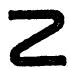
\includegraphics[keepaspectratio]{images/part002_45bf5402.jpg}}

Remark. When the set H satisfies the conditions of Proposition 2, it is a lattice with respect to the ordering \(f \leqslant g\) . But it should be remarked that a subset H of C can be a lattice with respect to this ordering without it being necessarily the case that the least upper bound (resp. greatest lower bound) in H of two functions u, v of H is the same as their least upper bound (resp. greatest lower bound) in C. * An example is provided by the convex mappings of a compact interval of R into R.*

COROLLARY. Suppose that H is such that, whenever \(u \in H\) and \(v \in H\) , we have sup \((u, v) \in H\) and inf \((u, v) \in H\) ; and is such that, given any two distinct points x, y of X and any two real numbers \(\alpha, \beta\) , there is a function \(g \in H\) such that \(g(x) = \alpha\) and \(g(y) = \beta\) . Then every continuous real-valued function on X can be uniformly approximated by functions belonging to H.

DEFINITION 1. If X is any set, a set H of mappings of X into a set Y is said to separate the elements of a subset A of X (or to be a separating set for the elements of A) if, given any two distinct elements x, y of A, there is a function \(f \in H\) such that \(f(x) \neq f(y)\) .

For example, if X is a completely regular space (Chapter IX, § 1, no. 5) then the set of all continuous mappings of X into {[}0, 1{]} separates the points of X.

THEOREM 2 (Stone). Let X be a compact space, and let H be a vector subspace of C(X; R) such that 1) the constant functions belong to H; 2) if \(u \in H\) , then \(|u| \in H\) ; 3) H separates the points of X. Then every continuous real-valued function on X can be uniformly approximated by functions of H.

It is enough to show that H satisfies the conditions of the Corollary to Proposition 2. By hypothesis, if \(u \in H\) and \(v \in H\) , we have

\[
\sup (u, v) = \frac {1}{2} (u + v + | u - v |) \in H
\]

and

\[
\inf (u, v) = \frac {1}{2} (u + v - | u - v |) \in H.
\]

On the other hand, let \(x\) and \(y\) be any two distinct points of \(X\) , and let \(\alpha, \beta\) be any two real numbers. By hypothesis, there is a function \(h \in H\) such that \(h(x) \neq h(y)\) : say \(h(x) = \gamma\) and \(h(y) = \delta\) . Since the constants belong to \(H\) , the function

\[
g (z) = \alpha + (\beta - \alpha) \frac {h (z) - \gamma}{\delta - \gamma}
\]

belongs to H and is such that \(g(x) = \alpha\) and \(g(y) = \beta\) .

\subsection{APPROXIMATION OF CONTINUOUS FUNCTIONS BY POLYNOMIALS}

Given a set H of real-valued functions defined on a set X, we say that a real-valued function defined on X is a polynomial (resp. a polynomial with no constant term) with real coefficients, in the functions of H, if it is of the form \(x \to g(f_{1}(x), f_{2}(x), \ldots, f_{n}(x))\) where g is a polynomial (resp. a polynomial with no constant term) in n indeterminates (n arbitrary) with real coefficients, and the \(f_{i}\) ( \(1 \leqslant i \leqslant n\) ) belong to H.

THEOREM 3 (Weierstrass-Stone). Let X be a compact space and let H be a set of continuous real-valued functions on X which separates the points of X. Then every continuous real-valued function on X can be uniformly approximated by polynomials (with real coefficients) in the functions of H.

An equivalent statement of the theorem is that any subalgebra of \(\mathcal{C}(\mathbf{X};\mathbf{R})\) which contains the constant functions and separates the points of \(\mathbf{X}\) is dense in \(\mathcal{C}(\mathbf{X};\mathbf{R})\) .

Let \(H_{0}\) be the set of all polynomials in the functions of H, and let \(\overline{H}_{0}\) be the closure of \(H_{0}\) in C. If g is any polynomial in n variables with real coefficients, then \((u_{1}, u_{2}, \ldots, u_{n}) \to g(u_{1}, u_{2}, \ldots, u_{n})\) is a continuous mapping of \(C^{n}\) into C, which maps \(H_{0}^{n}\) into \(H_{0}\) , and therefore maps \(\overline{H}_{0}^{n}\) into \(\overline{H}_{0}\) (Chapter I, § 2, no. 1, Theorem 1). In particular, \(\overline{H}_{0}\) is a vector subspace of C and evidently satisfies the first and third conditions of Theorem 2; we shall show that it also satisfies the second condition, and this will prove that \(\overline{H}_{0} = C\) .

Since every function \(u \in \overline{\mathbf{H}}_0\) is bounded in \(\mathbf{X}\) , it is enough to prove the following lemma:

LEMMA 1. For each real number \(\varepsilon > 0\) and each compact interval \(\mathbf{I} \subset \mathbf{R}\) there exists a polynomial \(p(t)\) with no constant term such that \(|p(t) - |t|| \leqslant \varepsilon\) for all \(t \in \mathbf{I}\) .

It is enough to prove the lemma for an interval of the form \(\mathbf{I} = [-a, +a]\) and hence, replacing \(t\) by \(at\) , for the interval \(\mathbf{I} = [-1, +1]\) . Since \(|t| = \sqrt{t^2}\) , Lemma 1 is a consequence of the following result:

LEMMA 2. Let \((P_n)\) be the sequence of polynomials without constant terms defined by

\[
p _ {0} (t) = 0, \quad p _ {n + 1} (t) = p _ {n} (t) + \frac {1}{2} (t - (p _ {n} (t)) ^ {2}), \quad n \geqslant 0.\tag{1}
\]

In the interval {[}0, 1{]} the sequence \((p_n)\) is increasing and converges uniformly to \(\sqrt{t}\) .

To prove Lemma 2 it is enough to show that, for all \(t \in [0, 1]\) , we have

\[
0 \leqslant \sqrt {t} - p _ {n} (t) \leqslant \frac {2 \sqrt {t}}{2 + n \sqrt {t}},\tag{2}
\]

for (2) implies that \(0 \leqslant \sqrt{t} - p_n(t) \leqslant 2 / n\) .

We prove (2) by induction on \(n\) . It is true for \(n = 0\) . If \(n \geqslant 0\) it follows from the inductive hypothesis (2) that \(0 \leqslant \sqrt{t} - p_n(t) \leqslant \sqrt{t}\) , hence \(0 \leqslant p_n(t) \leqslant \sqrt{t}\) , and therefore from (1) we have

\[
\sqrt {t} - p _ {n + 1} (t) = (\sqrt {t} - p _ {n} (t)) \left(1 - \frac {1}{2} (\sqrt {t} + p _ {n} (t))\right),
\]

so that \(\sqrt{t} - p_{n+1}(t) \geqslant 0\) , and from (2)

\[
\begin{array}{r l} \sqrt {t} - p _ {n + 1} (t) & \leqslant \frac {2 \sqrt {t}}{2 + n \sqrt {t}} \left(1 - \frac {\sqrt {t}}{2}\right) \leqslant \frac {2 \sqrt {t}}{2 + n \sqrt {t}} \left(1 - \frac {\sqrt {t}}{2 + (n + 1) \sqrt {t}}\right) \\ & = \frac {2 \sqrt {t}}{2 + (n + 1) \sqrt {t}}. \end{array} \tag {Q.E.D.}
\]

If X is not compact, the conclusion of Theorem 3 is not necessarily valid. For example, a continuous real-valued function on R which is bounded and not constant cannot be uniformly approximated in R by polynomials (cf.~Exercise 6).

PROPOSITION 3. Let \((\mathbf{K}_t)_{t \in \mathbf{I}}\) be a family of compact intervals of \(\mathbf{R}\) , \(\mathbf{K} = \prod_{t \in \mathbf{I}} \mathbf{K}_t\) their product, and let \(\mathbf{X}\) be a compact subspace of \(\mathbf{K}\) . Then every continuous real-valued function on \(\mathbf{X}\) can be uniformly approximated by polynomials in the coordinates \(x_t = \mathrm{pr}_t x\) .

For if \(x = (x_{t})\) and \(y = (y_{t})\) are two distinct points of X, there is at least one index t such that \(x_{t} \neq y_{t}\) ; hence the family of continuous functions \(pr_{t}\) satisfies the conditions of Theorem 3.

PROPOSITION 4. Let X be a compact space, let A be a closed subspace of X, and let H be a set of continuous real-valued functions on X which separates the points of \(\mathbb{C}A\) and is such that A is the intersection of the sets \(\overline{u}^{1}(0)\) as u runs through H. Then every continuous real-valued function on X which is zero on A can be uniformly approximated by polynomials without constant terms in the functions of H.

Consider first the particular case in which A consists of a single point \(x_{0}\) . The hypotheses then imply that H separates the points of X; for, if \(x \neq x_{0}\) , then by hypothesis there is a function \(u \in H\) such that \(u(x) \neq 0 = u(x_{0})\) . Hence, for each \(\varepsilon > 0\) and each continuous real-valued function f on X such that \(f(x_{0}) = 0\) , there exists (Theorem 3) a polynomial g in the functions of H such that \(|f(x) - g(x)| \leqslant \varepsilon\) for all \(x \in X\) . In particular \(|g(x_{0})| \leqslant \varepsilon\) , so that

\[
\left| f (x) - \left(g (x) - g \left(x _ {0}\right)\right) \right| \leqslant 2 \varepsilon
\]

for all \(x \in \mathbf{X}\) ; and since \(g(x) - g(x_0)\) is a polynomial in the functions of \(\mathbf{H}\) with no constant term, the result is established in this case.

In the general case, consider the equivalence relation R on X whose classes are the set A and the sets \(\{x\}\) for \(x \notin A\) . The quotient space X/R is Hausdorff (Chapter I, § 8, no. 6, Proposition 15) and therefore compact. Let \(\varphi: X \to X/R\) be the canonical mapping. Every continuous real-valued function f on X which vanishes on A can be written in the form \(f = f_{1} \circ \varphi\) , where \(f_{1}\) is a continuous real-valued function on X/R which vanishes at the point \(x_{0}' = \varphi(A)\) . Applying the result already proved to the space X/R and the point \(x_{0}'\) , we obtain the final result.

\subsection{APPLICATION: APPROXIMATION OF CONTINUOUS REAL-VALUED FUNCTIONS DEFINED ON A PRODUCT OF COMPACT SPACES}

THEOREM 4. Let \((\mathbf{X}_t)_{t\in \mathbf{I}}\) be a family of compact spaces, and let

\[
\mathrm{X} = \prod_ {t \in \mathrm{I}} \mathrm{X} _ {t}.
\]

Then every continuous real-valued function on X can be uniformly approximated by sums of a finite number of functions of the form

\[
(x _ {t}) \rightarrow \prod_ {\alpha \in \mathbf {J}} u _ {\alpha} (x _ {\alpha}),
\]

where J is an (arbitrary) finite subset of I and \(u_{\alpha}\) is a continuous real-valued function on \(X_{\alpha}\) for each \(\alpha \in J\) .

Consider the set H of ``functions of one variable'' \((x_{t}) \rightarrow u_{\alpha}(x_{\alpha})\) (any \(\alpha \in I\) ) which are continuous on X. This set separates the points of X, for if \(x = (x_{t})\) and \(y = (y_{t})\) are any two distinct points of X, there exists \(\alpha \in I\) such that \(x_{\alpha} \neq y_{\alpha}\) and there exists a continuous real-valued function \(h_{\alpha}\) on \(X_{\alpha}\) such that \(h_{\alpha}(x_{\alpha}) \neq h_{\alpha}(y_{\alpha})\) . The function \(x \rightarrow h_{\alpha}(\operatorname{pr}_{\alpha} x)\) then belongs to H and takes distinct values at x and y. Since every polynomial in the functions of H is of the form stated in the theorem, the result follows from Theorem 3.

If not all the \(X_{t}\) are compact, the conclusion of Theorem 4 is not necessarily valid (cf.~Exercise 9).

\subsection{APPROXIMATION OF CONTINUOUS MAPPINGS OF A COMPACT SPACE INTO A NORMED SPACE}

Let X be a compact space and let Y be a normed vector space over the field R (Chapter IX, § 3); the space \(\mathcal{C}(\mathbf{X};\mathbf{Y})\) will always be assumed to carry the topology of uniform convergence defined by the norm \(||u|| = \sup_{x\in \mathbf{X}}||u(x)||\) (§ 3, no. 2).

Given a set \(\mathbf{H}\) of continuous real-valued functions defined on \(\mathbf{X}\) , a finite family \((u_i)_{1\leqslant i\leqslant n}\) of functions belonging to \(\mathbf{H}\) , and a finite family \((a_i)_{1\leqslant i\leqslant n}\) of points of \(\mathbf{Y}\) : the mapping \(x\to \sum_{i = 1}^{n}a_iu_i(x)\) of \(\mathbf{X}\) into \(\mathbf{Y}\) is then continuous; we denote it by \(\sum_{i = 1}^{n}a_iu_i\) , and we say that it is a linear combination of functions of \(\mathbf{H}\) with coefficients in \(\mathbf{Y}\) . We say that a continuous mapping \(f:\mathbf{X}\rightarrow \mathbf{Y}\) can be uniformly approximated by linear combinations of functions of \(\mathbf{H}\) (with coefficients in \(\mathbf{Y}\) ), if \(f\) lies in the closure of the vector subspace of \(\mathcal{C}(\mathbf{X};\mathbf{Y})\) formed by these linear combinations.

PROPOSITION 5. Let X be a compact space, Y a normed space over R and H a subset of C (X; R). If every continuous real-valued function on X can be uniformly approximated by functions of H, then every continuous mapping f of X into Y can be uniformly approximated by linear combinations of functions of H with coefficients in Y.

Given any real number \(\varepsilon > 0\) , for each \(x \in \mathbf{X}\) there exists an open neighbourhood of \(x\) in which the oscillation of \(f\) is \(\leqslant \varepsilon\) . Hence there is a finite open covering \((\mathrm{A}_i)_{1 \leqslant i \leqslant n}\) of \(\mathbf{X}\) such that the oscillation of \(f\) in each \(\mathrm{A}_i\) is \(\leqslant \varepsilon\) . Let \(\boldsymbol{a}_i\) be a value of \(f\) in \(\mathrm{A}_i\) ( \(1 \leqslant i \leqslant n\) ), and let \((u_i)_{1 \leqslant i \leqslant n}\) be a continuous partition of unity subordinate to the covering \((\mathrm{A}_i)\) (Chapter IX, § 4, no. 4, Corollary to Proposition 4). Let \(x\) be any point of \(\mathbf{X}\) . For each index \(i\) such that \(x \notin \mathrm{A}_i\) , we have \(u_i(x) = 0\) , and for each index \(i\) such that \(x \in \mathrm{A}_i\) we have \(||f(x) - a_i|| \leqslant \varepsilon\) ; it follows that

\[
\left\| \boldsymbol {f} (x) - \sum_ {i = 1} ^ {n} \boldsymbol {a} _ {i} u _ {i} (x) \right\| = \left\| \sum_ {i = 1} ^ {n} (\boldsymbol {f} (x) - \boldsymbol {a} _ {i}) u _ {i} (x) \right\| \leqslant \varepsilon \sum_ {i = 1} ^ {n} u _ {i} (x) = \varepsilon .
\]

On the other hand, by hypothesis there is a function \(v_{i} \in \mathbf{H}\) such that

\[
\left| u _ {i} (x) - v _ {i} (x) \right| \leqslant \frac {\varepsilon}{\sum_ {j = 1} ^ {n} | | \boldsymbol {a} _ {j} | |}
\]

for all \(x \in \mathbf{X} (1 \leqslant i \leqslant n)\) ; hence we have

\[
\left\| \boldsymbol {f} (x) - \sum_ {i = 1} ^ {n} \boldsymbol {a} _ {i} v _ {i} (x) \right\| \leqslant 2 \varepsilon \text {   for   all   } x \in \mathbf {X},
\]

and the proof is complete.

From Proposition 5 it follows that, to each of the propositions in which we have proved that a certain subset H of C(X; R) is dense, there corresponds an analogous proposition for continuous mappings of X into an arbitrary normed space Y. We shall write down explicitly only the proposition which corresponds in this way to Theorem 3. Given a set H of real-valued functions on X, a polynomial in the functions of H, with coefficients in Y, is defined to be any linear combination, with coefficients in Y, of products of a finite (possibly empty) family of functions belonging to H. Then:

PROPOSITION 6. Let X be a compact space and let H be a set of continuous real-valued functions on X which separates the points of X. Then every continuous mapping of X into a normed space Y over R can be uniformly approximated by polynomials in the functions of H with coefficients in Y.

From this we deduce :

PROPOSITION 7. Let X be a compact space and let H be a set of continuous complex-valued functions on X which separates the points of X. Then every continuous mapping of X into a normed space Y over C can be uniformly approximated by polynomials in the functions \(f \in \mathbf{H}\) and their conjugates \(\overline{f}\) with coefficients in Y.

We have only to note that Y is also a normed space over R and to apply Proposition 6 to the set of real parts and imaginary parts of the functions \(f \in H\) , using the formulas

\[
\mathfrak {R} f = \frac {1}{2} (f + \overline {{f}}), \quad \Im f = \frac {1}{2 i} (f - \overline {{f}}).
\]

COROLLARY 1. If X is a compact subset of the space \(\mathbf{C}^n\) , then every continuous mapping \((z_1, z_2, \ldots, z_n) \to f(z_1, z_2, \ldots, z_n)\) of X into a normed space Y over the field C can be uniformly approximated by polynomials in the \(z_k\) and \(\overline{z}_k\) with coefficients in Y.

\pandocbounded{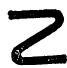
\includegraphics[keepaspectratio]{images/part002_94458643.jpg}}

We shall see later that in general it is not possible to approximate f uniformly by polynomials (with coefficients in Y) in the variables \(z_{k}\) alone, even if Y = C.

COROLLARY 2. Let X be a locally compact space and let \(\mathcal{C}_0(\mathbf{X})\) be the normed C-algebra of continuous mappings of X into C which tend to 0 at infinity. Let A be a subalgebra of \(\mathcal{C}_0(\mathbf{X})\) which separates the points of X and is such that (i) \(\overline{f} \in \mathbf{A}\) whenever \(f \in \mathbf{A}\) , (ii) for each \(x \in \mathbf{X}\) , there is an \(f \in \mathbf{A}\) such that \(f(x) \neq 0\) . Then A is dense in \(\mathcal{C}_0(\mathbf{X})\) .

If \(X'\) is the compact space obtained by adjoining a point at infinity \(\omega\) to X, then \(\mathcal{C}_{0}(\mathbf{X})\) can be identified with the subspace of \(\mathcal{C}(\mathbf{X};\mathbf{C})\) consisting of continuous mappings which vanish at \(\omega\) , the norm on \(\mathcal{C}_{0}(\mathbf{X})\) being defined by

\[
\left| \left| f \right| \right| = \sup _ {x \in \mathbf {X}} | f (x) | = \sup _ {x \in \mathbf {X}'} | f (x) |.
\]

By virtue of Proposition 7, every \(f \in \mathcal{C}_{0}(X)\) can be uniformly approximated by polynomials with complex coefficients in the functions belonging to A; moreover, since \(f(\omega) = 0\) , the argument of no. 2, Proposition 4 shows that we may suppose these polynomials to have no constant term, and then they belong to A.

Another application of Proposition 7 is the following :

PROPOSITION 8. Let P be the set of all periodic continuous mappings of \(\mathbf{R}^m\) into \(\mathbf{C}\) whose group of periods contains \(\mathbf{Z}^m\) . Then every function belonging to P can be uniformly approximated in \(\mathbf{R}^m\) by linear combinations, with complex coefficients, of functions of the form

\[
(x _ {1}, x _ {2}, \dots , x _ {m}) \rightarrow e (h _ {1} x _ {1} + h _ {2} x _ {2} + \dots + h _ {m} x _ {m}),
\]

where the \(h_{i}\) are rational integers (such linear combinations are called trigonometric polynomials in m variables).

We have only to observe that P (endowed with the topology of uniform convergence) is canonically isomorphic to the space of all continuous mappings of the compact space \(T^{m}\) into C (Chapter VII, § 1, no. 6), and apply Proposition 7 to the set of mappings of \(T^{m}\) into C which correspond to the m mappings \((x_{1}, x_{2}, \ldots, x_{m}) \to e(x_{i}) \quad (1 \leqslant i \leqslant m)\) of \(R^{m}\) into C.

\ExerciseGroupsStart

\ExerciseSection

\begin{enumerate}
\def\labelenumi{\arabic{enumi})}
\tightlist
\item
  Let X be a set, let Y be a uniform space containing more than one point, and let S be a non-empty set of non-empty subsets of X. Let \(Y' \subset \mathcal{F}(X; Y)\) be the set of all constant mappings of X into Y. For each \(y \in Y\) , let \(c_{y}\) be the constant mapping of X into Y whose value is y.
\end{enumerate}

\begin{enumerate}
\def\labelenumi{\alph{enumi})}
\item
  Show that \(y \to c_{y}\) is an isomorphism of Y onto the uniform subspace \(Y'\) of \(\mathcal{F}_{\mathfrak{S}}(\mathbf{X}; \mathbf{Y})\) .
\item
  \(\mathcal{F}_{\mathfrak{S}}(\mathbf{X};\mathbf{Y})\) is Hausdorff if and only if Y is Hausdorff and \(\mathfrak{S}\) is a covering of X.
\item
  \(\mathbf{Y}'\) is closed in \(\mathcal{F}_{\mathfrak{S}}(\mathbf{X};\mathbf{Y})\) if and only if \(\mathcal{F}_{\mathfrak{S}}(\mathbf{X};\mathbf{Y})\) is Hausdorff.
\end{enumerate}

\begin{enumerate}
\def\labelenumi{\arabic{enumi})}
\setcounter{enumi}{1}
\tightlist
\item
  Let X be a set, let Y be a Hausdorff uniform space containing more than one point, and let \(\mathfrak{S}_1, \mathfrak{S}_2\) be two sets of subsets of X which satisfy conditions \((\mathrm{F}_{\mathrm{I}}^{\prime}), (\mathrm{F}_{\mathrm{II}}^{\prime})\) of no. 2. Show that if \(\mathfrak{S}_1 \subset \mathfrak{S}_2\) and \(\mathfrak{S}_1 \neq \mathfrak{S}_2\) , then the uniformity of \(\mathfrak{S}_1\) -convergence is strictly coarser than the uniformity of \(\mathfrak{S}_2\) -convergence. In particular:
\end{enumerate}

\begin{enumerate}
\def\labelenumi{(\roman{enumi})}
\item
  If X is a non-compact Hausdorff topological space, the uniformity of compact convergence is strictly coarser than the uniformity of uniform convergence.
\item
  If X is a Hausdorff topological space which has infinite compact subsets (cf.~Chapter I, § 9, Exercise 4), then the uniformity of pointwise convergence is strictly coarser than the uniformity of compact convergence.
\end{enumerate}

\begin{enumerate}
\def\labelenumi{\arabic{enumi})}
\setcounter{enumi}{2}
\item
  Let X be a set, let S be a covering of X, let Y be a non-Hausdorff uniform space and let \(Y_{0}\) be the Hausdorff uniform space associated with Y (Chapter II, § 3, no. 8). Show that the Hausdorff uniform space associated with \(\mathcal{F}_{\mathfrak{S}}(\mathrm{X};\mathrm{Y})\) is isomorphic to \(\mathcal{F}_{\mathfrak{S}}(\mathrm{X};\mathrm{Y}_{0})\) .
\item
  Show that, on the set \(\mathcal{C}(\mathbf{R};\mathbf{R})\) of finite continuous real-valued functions defined on \(\mathbf{R}\) , the topology of uniform convergence with respect to the additive uniformity of R is not the same as the topology of uniform convergence with respect to the uniformity induced on R by the (unique) uniformity of the extended line \(\overline{R}\) (although the topologies induced by these two uniformities on R are the same).
\item
  Let X be a topological space. A set S of subsets of X is said to be saturated if it satisfies conditions \((\mathbf{F}_{\mathbf{I}}^{\prime})\) and \((\mathbf{F}_{\mathbf{II}}^{\prime})\) of no. 2 and if the closure of every set of S belongs to S.
\end{enumerate}

\begin{enumerate}
\def\labelenumi{\alph{enumi})}
\item
  Show that if X is normal and if S is saturated and covers X, then the set C(X; R) is dense in the space \(\tilde{\mathcal{C}}_{\mathfrak{S}}(X; \mathbf{R})\) (no. 6, Theorem 2, Corollary 2) with respect to the topology of S-convergence. In particular, C(X; R) is dense in \(F_{s}(X; \mathbf{R})\) . C(X; R) is closed in \(F_{s}(X; \mathbf{R})\) only if X is discrete.
\item
  Let X be a completely regular space (Chapter IX, § 1, no. 5) and let \(\mathfrak{S}_1, \mathfrak{S}_2\) be two saturated sets of subsets of X, such that \(\mathfrak{S}_1 \subset \mathfrak{S}_2\) and \(\mathfrak{S}_1 \neq \mathfrak{S}_2\) . Show that the topology of \(\mathfrak{S}_1\) -convergence on \(\mathcal{C}(\mathbf{X}; \mathbf{R})\) is strictly coarser than the topology of \(\mathfrak{S}_2\) -convergence.
\end{enumerate}

\begin{enumerate}
\def\labelenumi{\arabic{enumi})}
\setcounter{enumi}{5}
\tightlist
\item
  \begin{enumerate}
  \def\labelenumii{\alph{enumii})}
  \tightlist
  \item
    Let X be a topological space, Y a uniform space, and let \(\Phi\) be a filter on the set \(\mathcal{C}(X;Y)\) which converges pointwise to a function \(u_{0}\) . Then \(u_{0}\) is continuous at a point \(x_{0}\in X\) if and only if, for each entourage V of Y and each set \(M\in\Phi\) , there is a neighbourhood U of \(x_{0}\) and a mapping \(u\in M\) such that \((u_{0}(x),u(x))\in V\) for all \(x\in U\) .
  \end{enumerate}
\end{enumerate}

\begin{enumerate}
\def\labelenumi{\alph{enumi})}
\setcounter{enumi}{1}
\tightlist
\item
  Let X be a quasi-compact space, Y a uniform space and \(\Phi\) a filter on \(\mathcal{C}(X;Y)\) which converges pointwise to a function \(u_{0}\) . Then \(u_{0}\) is continuous on X if and only if, for each entourage V of Y and each set \(M\in\Phi\) , there exists a finite number of functions \(u_{i}\in\mathbf{M}(1\leqslant i\leqslant n)\) such that, for each \(x\in X\) , we have \((u_{0}(x),u_{i}(x))\in V\) for at least one index i.
\end{enumerate}

\begin{enumerate}
\def\labelenumi{\arabic{enumi})}
\setcounter{enumi}{6}
\tightlist
\item
  Let X, Y be two Hausdorff uniform spaces. For each continuous mapping \(f: \mathbf{X} \to \mathbf{Y}\) , let \(\mathbf{G}(f) \subset \mathbf{X} \times \mathbf{Y}\) be the graph of \(f\) ; \(\mathbf{G}(f)\) is closed in \(\mathbf{X} \times \mathbf{Y}\) (Chapter I, § 8, no. 1, Proposition 2, Corollary 2): hence \(f \to \mathbf{G}(f)\) is an injective mapping of \(\mathcal{C}(\mathbf{X}; \mathbf{Y})\) into the set \(\mathfrak{F}(\mathbf{X} \times \mathbf{Y})\) of non-empty closed subsets of \(\mathbf{X} \times \mathbf{Y}\) .
\end{enumerate}

\begin{enumerate}
\def\labelenumi{\alph{enumi})}
\item
  Show that the mapping \(f \to \mathbf{G}(f)\) of \(\mathcal{C}_u(\mathbf{X};\mathbf{Y})\) into \(\mathfrak{F}(\mathbf{X}\times \mathbf{Y})\) is uniformly continuous when \(\mathfrak{F}(\mathbf{X}\times \mathbf{Y})\) carries the uniformity defined in Chapter II, § 1, Exercise 5.
\item
  Let \(\Gamma\) be the image of \(\mathcal{C}(\mathbf{X};\mathbf{Y})\) in \(\mathfrak{F}(\mathbf{X}\times \mathbf{Y})\) under the mapping \(f\to \mathbf{G}(f)\) , and let \(\varphi :\Gamma \to \mathcal{C}_u(\mathbf{X};\mathbf{Y})\) be the inverse mapping. Show that if \(\mathbf{X}\) is compact, then \(\varphi\) is continuous on \(\Gamma\) (argue by contradiction).
\item
  Take both X and Y to be the compact interval {[}0, 1{]} of R. Show that \(\varphi\) is not uniformly continuous on \(\Gamma\) .
\end{enumerate}

\begin{enumerate}
\def\labelenumi{\arabic{enumi})}
\setcounter{enumi}{7}
\tightlist
\item
  Let X, Y be two metric spaces and let \((f_{n})\) be a sequence of Borel mappings of class \(\alpha\) of X into Y (Chapter IX, § 6, Exercise 16).
\end{enumerate}

\begin{enumerate}
\def\labelenumi{\alph{enumi})}
\item
  Suppose that the sequence \((f_{n})\) converges pointwise to a mapping f: X → Y. Show that f is of class \(\alpha + 1\) . {[}If U is an open subset of Y, note that \(\overline{f}^{1}(U) = \bigcup_{n \geqslant 1} \left( \bigcap_{k \geqslant 0} \overline{f}_{n+k}^{1}(U) \right)\) , and use Chapter IX, § 6, Exercise 4.{]}
\item
  Suppose that the sequence \((f_n)\) converges uniformly to \(f\) . Show that \(f\) is of class \(\alpha\) . {[}Let \(\mathbf{F}\) be a closed subset of \(\mathbf{Y}\) , and for each integer \(n > 0\) , let \(\mathbf{V}_n\) be the set of points of \(\mathbf{Y}\) whose distance from \(\mathbf{F}\) is \(\leqslant 1/n\) . Show that there is an increasing sequence \(n \to m(n)\) of integers such that \(\overline{f}^1(\mathbf{F}) = \bigcap_{n} \overline{f}_{m(n)}^1(\mathbf{V}_n)\) .{]}
\item
  Suppose that Y is of countable type. Show that, if \(f: X \to Y\) is a Borel function of class \(\alpha > 0\) , there exists a sequence of Borel functions \(g_{n}: X \to Y\) , of class \(<\alpha\) , such that \((g_{n})\) converges pointwise to f.~{[}Show that we may take the \(g_{n}\) to be functions which take only a finite number of values; use Exercises 4 h) and 16 c) of Chapter IX, § 6.{]}
\end{enumerate}

\begin{enumerate}
\def\labelenumi{\arabic{enumi})}
\setcounter{enumi}{8}
\item
  Let X be a Baire space, Y a metric space and \((f_{n})\) a sequence of continuous mappings of X into Y which converges pointwise to a function f.~A point \(x \in X\) is said to be a point of uniform convergence of the sequence \((f_{n})\) if, for each \(\varepsilon > 0\) , there exists a neighbourhood V of x and an integer p such that \(d(f_{m}(y), f_{n}(y)) \leqslant \varepsilon\) for all \(y \in V\) and all integers \(m \geqslant p, n \geqslant p, d\) being the metric on Y. Show that the complement S of the set of points of uniform convergence of the sequence \((f_{n})\) is meagre in X {[}cf.~Chapter IX, § 5, Exercise 22 a{]}. Give an example where S is dense in X. {[}Take X = Y = R, let \(n \to r_{n}\) be a bijection of N onto Q, and let \((g_{n})\) be a sequence of continuous mappings of R into {[}0, 1{]} which converges to the zero function for \(x \neq 0\) and to 1 at x = 0, the convergence being uniform in every open set of R which does not contain 0. Then consider the sequence of functions \(f_{n}(x) = \sum_{p=0}^{\infty} \alpha_{p} g_{n}(x - r_{p})\) , where the sequence \((\alpha_{p})\) tends to 0 in a suitable way.{]}
\item
  Show that, on the group \(\Gamma\) of homeomorphisms of the real line \(\mathbf{R}\) onto itself, the topology of pointwise convergence is the same as the topology of compact convergence (cf.~§ 3, Exercise 14).
\item
  Let X be a topological space and G a topological group. The set C(X; G) of continuous mappings of X into G is a subgroup of the group \(G^{X}\) . Let S be a set of subsets of X.
\end{enumerate}

\begin{enumerate}
\def\labelenumi{\alph{enumi})}
\item
  Suppose that for each \(A \in S\) , each neighbourhood V of e in G and each \(u \in C(X; G)\) , there exists a neighbourhood W of e in G such that \(sWs^{-1} \subset W\) for all \(s \in u(A)\) . Show that the topology of S-convergence is then compatible with the group structure of \(\mathcal{C}(X; G)\) , and that the right (resp. left) uniformity of the topological group \(\mathcal{C}_{\mathfrak{S}}(X; G)\) so defined is the same as the uniformity of S-convergence. Consider the case of pointwise convergence, the case of compact convergence when G is locally compact, and the case where G is abelian.
\item
  If G is the group \(\mathbf{SL}(2, \mathbf{R})\) endowed with the topology induced by that of \(R^{4}\) , show that the topology of uniform convergence is not compatible with the group structure of \(\mathcal{C}(\mathbf{R}; \mathbf{G})\) .
\end{enumerate}

\begin{enumerate}
\def\labelenumi{\arabic{enumi})}
\setcounter{enumi}{11}
\tightlist
\item
  Let X be a topological space and let A be a topological ring (Chapter III, § 6, no. 3). The set C(X; A) of continuous mappings of X into A is a subring of the ring A\^{}X. Let S be a set of subsets of X.
\end{enumerate}

\begin{enumerate}
\def\labelenumi{\alph{enumi})}
\item
  Suppose that, for each \(\mathbf{M} \in \mathfrak{S}\) and each \(u \in \mathcal{C}(\mathbf{X}; \mathbf{A})\) , the set \(u(\mathbf{M})\) is bounded (Chapter III, § 6, Exercise 12). Show that the topology of \(\mathfrak{S}\) -convergence is compatible with the ring structure of \(\mathcal{C}(\mathbf{X}; \mathbf{A})\) . Consider the case of pointwise convergence and the case of compact convergence.
\item
  Let X be a locally compact \(\sigma\) -compact space which is not compact (Chapter I, § 9, no. 9). Show that the topology of uniform convergence is not compatible with the ring structure of \(\mathcal{C}\) (X; R).
\end{enumerate}

\ExerciseSection

\begin{enumerate}
\def\labelenumi{\arabic{enumi})}
\item
  Let \(f\) be the real-valued function on \(\mathbf{R}\) which is equal to \(0\) for \(x \leqslant 0\) , to \(x\) for \(0 \leqslant x \leqslant 1\) , and to \(1\) for \(x \geqslant 1\) . Show that the sequence of real-valued functions \(f_n(x) = f(nx - n^2)\) ( \(n \in \mathbf{N}\) ) is equicontinuous but not uniformly equicontinuous on \(\mathbf{R}\) , although it is formed of uniformly continuous functions.
\item
  Let X be a Hausdorff topological space in which every point admits a countable fundamental system of neighbourhoods, and let Y be a uniform space. Let H be a subset of \(\mathcal{C}(X;Y)\) with the property that, for each compact subset K of X, the set \(H|K\) of restrictions to K of mappings \(u\in H\) is an equicontinuous subset of \(\mathcal{C}(K;Y)\) . Show that H is equicontinuous (argue by contradiction).
\item
  Let X, Y, Z be three metric spaces and let H be a subset of \(\mathcal{C}(X \times Y; Z)\) . Suppose that, for each \(x_{0} \in X\) , the set of mappings \(u(x_{0}, .)\) , as u runs through H, is an equicontinuous subset of \(\mathcal{C}(Y; Z)\) , and that, for each \(y_{0} \in Y\) , the set of mappings \(u(., y_{0})\) , as u runs through
\end{enumerate}

H, is an equicontinuous subset of \(\mathcal{C}\) (X; Z). Show that if X is complete, then for each \(b \in \mathbf{Y}\) there is a set \(S_b\) in X whose complement is meagre in X and which is such that, for each \(a \in \mathbf{S}_b\) , the set H is equicontinuous at \((a, b)\) . (Apply Chapter IX, § 5, Exercise 23, using Chapter X, § 2, Proposition 1, Corollary 1.)

\begin{enumerate}
\def\labelenumi{\arabic{enumi})}
\setcounter{enumi}{3}
\tightlist
\item
  Let X, Y, Z be three uniform spaces.
\end{enumerate}

\begin{enumerate}
\def\labelenumi{\alph{enumi})}
\item
  Let H be a uniformly equicontinuous subset of \(\mathcal{C}(\mathrm{Y};\mathrm{Z})\) . If H, \(\mathcal{C}(\mathrm{X};\mathrm{Y})\) and \(\mathcal{C}(\mathrm{X};\mathrm{Z})\) are endowed with the uniformity of uniform convergence, show that the mapping \((u,v)\to u\circ v\) of \(\mathrm{H}\times \mathcal{C}(\mathrm{X};\mathrm{Y})\) into \(\mathcal{C}(\mathrm{X};\mathrm{Z})\) is uniformly continuous.
\item
  Let K be a uniformly equicontinuous subset of \(\mathcal{C}(\mathbf{X};\mathbf{Y})\) , and let L be a uniformly equicontinuous subset of \(\mathcal{C}(\mathbf{Y};\mathbf{Z})\) . Show that the set of mappings \(v \circ u\) , where u runs through K and v runs through L, is a uniformly equicontinuous subset of \(\mathcal{C}(\mathbf{X};\mathbf{Z})\) .
\end{enumerate}

\begin{enumerate}
\def\labelenumi{\arabic{enumi})}
\setcounter{enumi}{4}
\item
  Let X be a topological space and let Y be a normed space over a non-discrete valued division ring K. Let H be a subset of \(\mathcal{F}(X;Y)\) , equicontinuous at a point \(x_{0}\in X\) , and let k\textgreater0 be a real number. Then the set \(H_{k}\) of linear combinations \(\sum_{i}c_{i}u_{i}\) of functions \(u_{i}\in H\) , such that \(\sum_{i}|c_{i}|\leqslant k\) , is equicontinuous at the point \(x_{0}\) .
\item
  Let X be a topological space, Y a uniform space, H an equicontinuous subset of \(\mathcal{C}(\mathbf{X};\mathbf{Y})\) , and \(\Phi\) a filter on H. Show that the set of all \(x\in X\) such that \(\Phi(x)\) is a Cauchy filter base on Y is closed in X.
\item
  Let X be a topological space, Y a complete Hausdorff uniform space, and let \(\varphi\) be a uniformly continuous homeomorphism of Y onto an open subset \(\varphi(Y)\) of a Hausdorff uniform space \(Y'\) . Let H be an equicontinuous subset of \(\mathcal{C}(X; Y)\) , and let \(H'\) be the set of mappings \(\varphi \circ u\) , where \(u \in H\) . If \(v\) lies in the closure of \(H'\) in \(\mathcal{F}_s(X; Y')\) , show that \(\overline{v}^{1}(\varphi(Y))\) is both open and closed in X. In particular, if X is connected, \(v(X)\) is contained in \(\varphi(Y)\) or in a connected component of \(\mathbb{C}\varphi(Y)\) . (Observe that \(v\) is continuous, and use Exercise 6.)
\item
  Let \(\mathbf{H}\) be an equicontinuous set of mappings of a topological space \(\mathbf{X}\) into \(\mathbf{R}\) .
\end{enumerate}

\begin{enumerate}
\def\labelenumi{\alph{enumi})}
\item
  Show that the set of upper (resp. lower) envelopes of finite subsets of H is equicontinuous.
\item
  Let v be a mapping of X into \(\overline{R}\) which lies in the closure of H with respect to the topology of pointwise convergence. Show that v is continuous on \(\mathbf{X}\) and that the sets \(\overline{v} (+\infty)\) and \(\overline{v} (-\infty)\) are both open and closed in \(\mathbf{X}\) (use Exercise 7).
\item
  Deduce from a) and b) that the upper (resp. lower) envelope w (resp. v) of H is continuous on X and that \(\overline{w}^{1}(+\infty)\) {[}resp. \(\overline{v}^{1}(-\infty)\) {]} is both open and closed in X.
\item
  Suppose that X is connected and that there is a point \(x_{0} \in X\) such that \(\mathbf{H}(x_{0})\) is bounded above in R. Show that, for every compact subset K of X, the set of restrictions to K of functions of H is uniformly bounded above in K {[}use c){]}.
\end{enumerate}

\begin{enumerate}
\def\labelenumi{\arabic{enumi})}
\setcounter{enumi}{8}
\item
  Let X be a set, Y a uniform space and S a covering of X. A subset H of the uniform space \(\mathcal{F}_{\mathfrak{S}}(\mathbf{X};\mathbf{Y})\) is precompact if and only if (i) for each \(x\in X\) , \(\mathbf{H}(x)\) is precompact in Y; (ii) the uniformity of S-convergence and that of pointwise convergence coincide on H. (Apply Theorem 2 by considering X as a discrete space and reducing to the case where Y is Hausdorff and complete.)
\item
  \begin{enumerate}
  \def\labelenumii{\alph{enumii})}
  \tightlist
  \item
    Let X be a compact space, let \((f_{n})\) be a sequence of continuous mappings \(X \rightarrow X\) , which converges pointwise but not uniformly in X to a continuous function (§ 1, no. 6, Remark 2). Show that the set of mappings \(f_{n}\) is relatively compact in \(\mathcal{C}_{s}(X; X)\) but not in
  \end{enumerate}
\end{enumerate}

\[
\mathcal {C} _ {u} (\mathrm{X}; \mathrm{X}) = \mathcal {C} _ {c} (\mathrm{X}; \mathrm{X}).
\]

\begin{enumerate}
\def\labelenumi{\alph{enumi})}
\setcounter{enumi}{1}
\tightlist
\item
  Let I be the interval \([-1, +1]\) of R and for each integer n \textgreater{} 0 let \(u_{n}(x) = \sin \sqrt{x + 4n^{2}\pi^{2}}\) for all \(x \geqslant 0\) . Show that the set H of functions \(u_{n}\) is an equicontinuous subset of \(\mathcal{C}(\mathbf{R}_{+}; \mathbf{I})\) and is relatively compact in \(\mathcal{C}_{c}(\mathbf{R}_{+}; \mathbf{I})\) but not in \(\mathcal{C}_{u}(\mathbf{R}_{+}; \mathbf{I})\) . (Note that the sequence \((u_{n})\) converges pointwise to 0.)
\end{enumerate}

\begin{enumerate}
\def\labelenumi{\arabic{enumi})}
\setcounter{enumi}{10}
\item
  Let X be a completely regular space and let S be a set of subsets of X whose interiors cover X. Show that the space \(\mathcal{C}_{s}(X;R)\) is not locally compact.
\item
  Let X be a topological space, Y a uniform space, H an equicontinuous subset of C(X; Y) and V a symmetric entourage of Y. Given a point \(x \in X\) , show that the set of points \(x' \in X\) for which there is an integer n (depending on \(x'\) ) such that \(\mathrm{H}(x') \subset \mathrm{V}^n(\mathrm{H}(x))\) is both open and closed in X. Deduce that, if K is any compact connected subset of X and if \(x_0\) is any point of K, there is an integer n \textgreater{} 0 such that \(\mathrm{H}(\mathrm{K}) \subset \mathrm{V}^n(\mathrm{H}(x_0))\) .
\end{enumerate}

¶ 13) Let X be a topological space, let Y be a locally compact uniform space and let H be an equicontinuous subset of C(X;Y).

\begin{enumerate}
\def\labelenumi{\alph{enumi})}
\item
  Let A be the set of all \(x \in X\) such that \(H(x)\) is relatively compact in Y. Show that A is open in X (cf.~Chapter I, § 9, no. 7, Proposition 10 and Chapter II, § 4, no. 3, Proposition 4).
\item
  Suppose in addition that Y is complete with respect to its uniformity; then A is also closed in X {[}observe that if \(x_{0} \in \overline{A}\) , then \(\mathrm{H}(x_{0})\) is relatively compact in Y by considering an ultrafilter on \(\mathrm{H}(x_{0})\) as the image of an ultrafilter on H{]}. In this case, if X is connected, then H is relatively compact in \(\mathcal{C}_{c}(\mathrm{X};\mathrm{Y})\) if and only if, for one point \(x_{0} \in X\) , the set \(\mathrm{H}(x_{0})\) is relatively compact in Y.
\item
  Take X to be the compact interval {[}0, 1{]} of R, and take Y to be the interval {]}0, 1{[} endowed with the uniformity induced by that of R. Give an example of an equicontinuous subset H of C (X; Y) such that the set A defined in a) is the interval {]}0, 1{]}.
\item
  Suppose that X = Y and that H consists of homeomorphisms of X onto itself. Show that if H is uniformly equicontinuous, then the set A defined in a) is both open and closed in X.
\end{enumerate}

\begin{enumerate}
\def\labelenumi{\arabic{enumi})}
\setcounter{enumi}{13}
\tightlist
\item
  Let \(\Gamma\) be an equicontinuous group of homeomorphisms of \(\mathbf{R}\) . Show that if a homeomorphism \(u \in \Gamma\) leaves at least one point of \(\mathbf{R}\) fixed, and if \(u\) is increasing, then \(u\) is the identity mapping (show that otherwise the group generated by \(u\) is not equicontinuous at a suitably chosen fixed point of \(u\) ). If \(u\) is decreasing, then \(u^2\) is the identity mapping.
\end{enumerate}

¶ 15) Let X be a compact metrizable space, let \(\Gamma\) be the group of all homeomorphisms of X, and let G be a subgroup of \(\Gamma\) which operates transitively on X. If H is the centralizer of G in \(\Gamma\) , show that H is equicontinuous. {[}Argue by reductio ad absurdum, supposing that H is not equicontinuous at some point \(a \in \mathbf{X}\) ; deduce the existence of a sequence of points \(x_n \in \mathbf{X}\) and a sequence of elements \(u_n \in \mathbf{H}\) such that

\[
\lim _ {n \rightarrow \infty} x _ {n} = a, \quad \lim _ {n \rightarrow \infty} u _ {n} (a) = b, \quad \lim _ {n \rightarrow \infty} u _ {n} (x _ {n}) = c,
\]

where \(b \neq c\) . Hence show that the sequence \((u_n)\) converges pointwise in \(X\) , but that no point of \(X\) is a point of uniform convergence of this sequence; this contradicts Exercise 9 of §1.{]}

\begin{enumerate}
\def\labelenumi{\arabic{enumi})}
\setcounter{enumi}{15}
\tightlist
\item
  Let X be a Hausdorff uniform space and let \(\Gamma\) be an equicontinuous group of homeomorphisms of X. The equivalence relation R defined by \(\Gamma\) on X is open (Chapter I, § 5, no. 2).
\end{enumerate}

\begin{enumerate}
\def\labelenumi{\alph{enumi})}
\item
  Show that if every orbit of \(\Gamma\) is closed in \(\mathbf{X}\) , then the orbit space \(\mathbf{X} / \Gamma\) is Hausdorff.
\item
  Show that if every orbit of \(\Gamma\) is compact, then the relation \(\mathbf{R}\) is closed (use Chapter I, § 5, no. 4, Proposition 10).
\item
  Give an example where X is compact but none of the orbits of \(\Gamma\) is closed in X (cf.~Chapter III, § 2, Exercise 29).
\end{enumerate}

¶ 17) Let X be a compact space and Γ a countable group of homeomorphisms of X. Suppose that the orbit space X/Γ is Hausdorff (and therefore compact).

\begin{enumerate}
\def\labelenumi{\alph{enumi})}
\item
  Show that, for each \(x \in \mathbf{X}\) , the orbit \(\Gamma(x)\) of \(x\) is finite (observe that if it were infinite it would have no isolated point, and use Baire's theorem (Chapter IX, § 5, no. 3, Theorem 1)).
\item
  For each \(x_0 \in \mathbf{X}\) , let \(\Delta(x_0)\) be the normal subgroup of \(\Gamma\) consisting of homeomorphisms which leave fixed all the points of the orbit \(\Gamma(x_0)\) . Show that if \(\Delta(x_0)\) is finitely generated, then \(\Gamma\) is equicontinuous at \(x_0\) . {[}Let \(f_i (1 \leqslant i \leqslant m)\) be the generators of \(\Delta(x_0)\) , and let \(g_k (1 \leqslant k \leqslant n)\) be representatives of each of the cosets of \(\Delta(x_0)\) in \(\Gamma\) other than \(\Delta(x_0)\) itself. Take a neighbourhood \(\mathbf{V}\) of \(x_0\) such that none of the sets \(f_i(\mathbf{V})\) , \(f_i^{-1}(\mathbf{V})\) meets any of the sets \(g_k(\mathbf{V})\) , and then use the fact that the equivalence relation defined by \(\Gamma\) is closed (Chapter I, § 10, no. 4, Proposition 8).{]}
\item
  Without making any hypothesis on \(\Delta(x_{0})\) , suppose that \(x_{0}\) has a countable fundamental system of connected neighbourhoods in X. Show that \(\Gamma\) is equicontinuous at \(x_{0}\) {[}same method as in b){]}. Deduce that if X is locally connected, then \(\Gamma\) is equicontinuous.
\item
  Take X to be the compact subspace of R consisting of the points 0, 1, 1/n and \(1 + 1/n\) (n an integer \(\geqslant 2\) ). Give an example of a countable group \(\Gamma\) of homeomorphisms of X, such that \(X/\Gamma\) is Hausdorff but \(\Gamma\) is not equicontinuous.
\end{enumerate}

¶ 18) Let G be a Hausdorff topological group operating continuously on a Hausdorff topological space X. G is said to be proper at a point \(x_{0} \in X\) if the orbit G. \(x_{0}\) is closed in X and if G operates properly on G. \(x_{0}\) (Chapter III, § 4, no. 1).

\begin{enumerate}
\def\labelenumi{\alph{enumi})}
\item
  Let G be a locally compact topological group operating continuously on a Hausdorff uniform space X. Suppose that the set of homeomorphisms \(x \rightarrow s.x\) of X, as s runs through G, is equicontinuous. Show that if G is proper at a point \(x_{0} \in X\) , then there is a neighbourhood V of \(x_{0}\) such that the set of elements \(s \in G\) such that \(s.V \cap V \neq \emptyset\) is relatively compact in G (cf.~Chapter III, § 4, no. 4, Proposition 7). Deduce that the set D of points of X at which G is proper is open in X and that G operates properly on D. If in addition X is locally compact, show that D is both open and closed in X (use no. 1, Proposition 1, Corollary 2).
\item
  In the real plane \(\mathbf{R}^2\) , let \(\mathbf{E}\) be the set consisting of the origin \((0,0)\) and the points \((0,2^{-n})\) as \(n\) runs through the integers \(\geqslant 0\) . For each \(n\in \mathbf{Z}\) such that \(n\neq 0\) let \(u_{n}\) be the restriction to \(\mathbf{E}\) of an affine linear mapping of \(\mathbf{R}^2\) into itself, such that \(u_{n}(0,0) = (n,0)\) , and \(u_{n}(0,2^{-|n|}) = (0,\theta^{n})\) where \(\theta\) is an irrational number such that \(0 <   \theta <  1\) . Let \(\mathbf{X}\) be the (locally compact) subspace of \(\mathbf{R}^2\) which is the union of \(\mathbf{E}\) and the sets \(u_{n}(\mathbf{E})\) for \(n\in \mathbf{Z},n\neq 0\) . Furthermore, let \(u_{0}\) denote the identity mapping of \(\mathbf{E}\) , and extend \(u_{n}(n\in \mathbf{Z})\) to the whole of \(\mathbf{X}\) by putting \(u_{n}(u_{m}(x)) = u_{n + m}(x)\) for all \(x\in \mathbf{E}\) and all \(m\in \mathbf{Z}\) . The set \(\mathbf{G}\) of mappings \(u_{n}\) is a group of homeomorphisms of \(\mathbf{X}\) which is given a discrete topology so that \(\mathbf{G}\) operates continuously on \(\mathbf{X}\) . Show that \(\mathbf{G}\) is proper at every point of \(\mathbf{X}\) , but is not equicontinuous and does not operate properly on \(\mathbf{X}\) .
\item
  Let X be the (not locally compact) subspace of \(R^{2}\) (identified with C) which is the union of the half-plane y \textgreater{} 0 and the origin. Define a homeomorphism u of X onto itself by putting \(u(0, 0) = (0, 0)\) and \(u(re^{i\omega}) = re^{i\omega'}\) where \(\omega' = \frac{1}{2}\omega\) if \(0 < \omega \leqslant \frac{1}{2}\pi\) , \(\omega' = \omega - \frac{1}{4}\pi\) for \(\frac{1}{2}\pi \leqslant \omega \leqslant \frac{3}{4}\pi\) , \(\omega' = 2\omega - \pi\) for \(\frac{3}{4}\pi \leqslant \omega < \pi\) (r \textless{} 0, \(0 < \omega < \pi\) ). Let G be the group of homeomorphisms of X generated by u, and endow G with the discrete topology. Show that G is equicontinuous on X and that the set of points of X at which G is proper is the half-plane y \textgreater{} 0.
\end{enumerate}

\begin{enumerate}
\def\labelenumi{\arabic{enumi})}
\setcounter{enumi}{18}
\tightlist
\item
  Let X be a Hausdorff uniform space and let G be a group of homeomorphisms of X onto itself.
\end{enumerate}

\begin{enumerate}
\def\labelenumi{\alph{enumi})}
\item
  Show that if \(\mathbf{G}\) is equicontinuous and discrete with respect to the topology of pointwise convergence, then \(\mathbf{G}\) is closed in \(\mathcal{F}_s(\mathbf{X};\mathbf{X})\) .
\item
  Show that if G, endowed with the discrete topology, is proper at one point of X at least (Exercise 18), then G is closed in \(\mathcal{F}_{s}(\mathbf{X};\mathbf{X})\) and the topology of pointwise convergence induces the discrete topology on G.
\item
  Let X be the topological sum of two spaces \(X_{1}, X_{2}\) , each homeomorphic to R, so that X can be identified with the product space \(R \times \{1, 2\}\) . Endow X with the product uniformity. For each pair \((m, n)\) of rational integers let \(u_{mn}\) denote the homeomorphism of X defined by \(u_{mn}(x_{1}) = x_{1} + m\alpha + n\beta\) , \(u_{mn}(x_{2}) = x_{2} + m\gamma + n\delta\) , where \(x_{1} \in X_{1}\) and \(x_{2} \in X_{2}\) , and \(\alpha, \beta, \gamma, \delta\) are four non-zero real numbers such that \(\alpha/\beta\) and \(\gamma/\delta\) are irrational and distinct. Show that the \(u_{mn}\) form a group of homeomorphisms of X which is equicontinuous and discrete with respect to the topology of pointwise convergence, but that G (with the discrete topology) is not proper at any point of X.
\end{enumerate}

\begin{enumerate}
\def\labelenumi{\arabic{enumi})}
\setcounter{enumi}{19}
\tightlist
\item
  Let G be a group of homeomorphisms of a Hausdorff uniform space X. Suppose that G is equicontinuous and that G, endowed with the discrete topology, operates properly on X. Suppose, furthermore, that the set of points \(x \in X\) , which are not fixed points of any homeomorphism \(u \in G\) other than the identity, is dense in X. Under these conditions, show that there is an open set F in X such that \(F \cap U(F) = \varnothing\) for all \(u \in G\) other than the identity, and such that the canonical image of F in the orbit space X/G is a dense open subset of X/G, homeomorphic to F (use Exercise 16 and Zorn's lemma).
\end{enumerate}

\ExerciseSection

\begin{enumerate}
\def\labelenumi{\arabic{enumi})}
\item
  Let X be a topological space and Y a metric space. Show that the set of all mappings of X into Y whose oscillation (Chapter IX, § 2, no. 3) at every point of X is \(\leqslant\alpha\) (where \(\alpha\) is a given real number \textgreater0) is closed in the space \(\mathcal{F}_{u}(\mathbf{X};\mathbf{Y})\) .
\item
  Let X be a set; show that the mapping \(u \to \sup_{x \in X} u(x)\) of \(\mathcal{B}(X; \mathbf{R})\) into R is continuous.
\item
  Let \(\mathbf{X}\) be a metric space, \(d\) the metric on \(\mathbf{X}\) . For each \(x \in \mathbf{X}\) let \(d_x\) be the real-valued function \(y \to d(x, y)\) which is continuous on \(\mathbf{X}\) . Show that the mapping \(x \to d_x\) is an isometry of \(\mathbf{X}\) onto a subspace of \(\mathcal{C}_u(\mathbf{X}; \mathbf{R})\) {[}endowed with the pseudometric \(\delta(u, v) = \sup_{x \in \mathbf{X}} |u(x) - v(x)|\) {]}.
\item
  A completely regular space X is such that the metrizable space \(\mathcal{C}_{u}(\mathbf{X};\mathbf{R})\) is of countable type if (and only if) X is compact and metrizable. {[}By considering the Stone-Čech compactification of X (Chapter IX, § 1, Exercise 7) show that X must be metrizable, and then observe that the space \(\mathcal{C}_{u}(\mathbf{Z};\mathbf{R})\) is not of countable type.{]}
\item
  Let X be a completely regular space.
\end{enumerate}

\begin{enumerate}
\def\labelenumi{\alph{enumi})}
\tightlist
\item
  If every point of the space \(\mathcal{C}_{c}(\mathbf{X};\mathbf{R})\) has a countable fundamental system of neighbourhoods, then there exists an increasing sequence \((\mathbf{K}_{n})\) of compact subsets of X such that every compact subset of X is contained in some \(K_{n}\) ; and \(\mathcal{C}_{c}(\mathbf{X};\mathbf{Y})\) is then metrizable for any metrizable space Y.
\item
  \(\mathcal{C}_{c}(\mathbf{X};\mathbf{R})\) is metrizable and of countable type if and only if all the compact subspaces \(K_{n}\) are metrizable (use Exercise 4). For every metrizable space Y of countable type, \(\mathcal{C}_{c}(\mathbf{X};\mathbf{Y})\) is then metrizable and of countable type.
\end{enumerate}

\begin{enumerate}
\def\labelenumi{\arabic{enumi})}
\setcounter{enumi}{5}
\tightlist
\item
  \begin{enumerate}
  \def\labelenumii{\alph{enumii})}
  \tightlist
  \item
    Let X be a topological space, Y a metric space, d the metric on Y, n an integer \textgreater0 and S a subset of the space \(X^{n} \times Y^{n} \times R_{+}^{*}\) . For each point \(z = ((x_{i}), (y_{i}), r) \in \mathbf{S}\) , let \(U_{z}\) be the open subset of \(\mathcal{C}_{s}(X; Y)\) consisting of continuous mappings f of X into Y such that \(d(f(x_i), y_i) < r\) for \(1 \leqslant i \leqslant n\) . Show that, if D is a dense subset of S, we have \(\bigcup_{z \in \mathbf{S}} \mathrm{U}_z = \bigcup_{z \in \mathbf{D}} \mathrm{U}_z\) .
  \end{enumerate}
\end{enumerate}

\begin{enumerate}
\def\labelenumi{\alph{enumi})}
\setcounter{enumi}{1}
\tightlist
\item
  Deduce from a) that if the topologies of X and Y have countable bases, then every subspace of \(\mathcal{C}_{s}(\mathbf{X};\mathbf{Y})\) is a Lindelöf space (Chapter I, § 9, Exercise 15) and is therefore paracompact (Chapter IX, § 4, Exercise 23).
\end{enumerate}

\begin{enumerate}
\def\labelenumi{\arabic{enumi})}
\setcounter{enumi}{6}
\item
  Let X be a space which has a countable dense subset, let Y be a Hausdorff space in which every point has a countable fundamental system of neighbourhoods (resp. a metrizable space) and let H be a subset of C(X; Y). Show that if C is a topology on H which is finer than the topology of pointwise convergence in X and with respect to which H is compact, then every point of H has a countable fundamental system of neighbourhoods in the topology C (resp. C is metrizable). (Note that if D is any countable dense subset of X, then the topology C is finer than the topology of pointwise convergence in D and that the latter topology is Hausdorff.)
\item
  \begin{enumerate}
  \def\labelenumii{\alph{enumii})}
  \tightlist
  \item
    Let \(f\) be the continuous mapping \((x, y) \to xy\) of \(\mathbf{R} \times \mathbf{R}\) into \(\mathbf{R}\) . Show that the mapping \(x \to f(x, .)\) of \(\mathbf{R}\) into \(\mathcal{C}_u(\mathbf{R}; \mathbf{R})\) is not continuous.
  \end{enumerate}
\end{enumerate}

\begin{enumerate}
\def\labelenumi{\alph{enumi})}
\setcounter{enumi}{1}
\tightlist
\item
  Let X, Y be two topological spaces, let Z be a uniform space and let \(f: \mathbf{X} \times \mathbf{Y} \to \mathbf{Z}\) be a mapping. Show that if \(f(x, .)\) is continuous on Y for all \(x \in \mathbf{X}\) and if the mapping \(x \to f(x, .)\) of X into \(\mathcal{C}_u(Y; \mathbf{Z})\) is continuous, then \(f\) is continuous on \(\mathbf{X} \times \mathbf{Y}\) .
\end{enumerate}

\begin{enumerate}
\def\labelenumi{\arabic{enumi})}
\setcounter{enumi}{8}
\tightlist
\item
  \begin{enumerate}
  \def\labelenumii{\alph{enumii})}
  \tightlist
  \item
    Let X, Y, Z be three topological spaces. Suppose that X and Y are Hausdorff and that every point of each of these spaces has a countable fundamental system of neighbourhoods. Let f be a mapping of \(X \times Y\) into Z such that \(f(x, .)\) is continuous on Y for each \(x \in X\) and such that the mapping \(x \to f(x, .)\) of X into \(\mathcal{C}_{c}(Y; Z)\) is continuous. Show that f is continuous on \(X \times Y\) (cf.~§1, no. 6, Theorem 2, Corollary 3).
  \end{enumerate}
\end{enumerate}

\begin{enumerate}
\def\labelenumi{\alph{enumi})}
\setcounter{enumi}{1}
\tightlist
\item
  Show that the conclusion of a) holds good when the hypothesis on X is replaced by the hypothesis that X is locally compact and Z is a uniform space (use § 2, Exercise 2, and Ascoli's theorem) {[}cf.~Exercise II b){]}.
\end{enumerate}

¶ 10) Let X, Y be two topological spaces. For each subset A of X and each subset B of Y let \(T(A, B)\) denote the set of all \(u \in \mathcal{C}(X; Y)\) such that \(u(A) \subset B\) .

Let \(\mathfrak{U} = (\mathbf{U}_{\alpha})\) be an open covering of \(\mathbf{X}\) . Let \(\mathfrak{G}_{\mathfrak{U}}\) denote the topology on \(\mathcal{C}(\mathbf{X};\mathbf{Y})\) generated by the sets \(T(\mathbf{F},\mathbf{V})\) , where \(\mathbf{V}\) runs through the set of all open sets of \(\mathbf{Y}\) and \(\mathbf{F}\) runs through the set of closed subsets of \(\mathbf{X}\) contained in at least one \(\mathbf{U}_{\alpha}\) .

\begin{enumerate}
\def\labelenumi{\alph{enumi})}
\item
  Show that \(\mathfrak{G}_{\mathfrak{U}}\) is finer than the compact-open topology (use Theorem 3 of Chapter IX, § 4, no. 3). If \(\mathbf{X}\) is regular, the mapping \((u, x) \to u(x)\) of \(\mathcal{C}(\mathbf{X}; \mathbf{Y}) \times \mathbf{X}\) into \(\mathbf{Y}\) is continuous when \(\mathcal{C}(\mathbf{X}, \mathbf{Y})\) carries the topology \(\mathfrak{G}_{\mathfrak{U}}\) .
\item
  Let \(\mathfrak{C}\) be a topology on \(\mathcal{C}(\mathbf{X};\mathbf{Y})\) with respect to which the mapping \((u,x)\to u(x)\) of \(\mathcal{C}(\mathbf{X};\mathbf{Y})\times \mathbf{X}\) into \(\mathbf{Y}\) is continuous. Let \(u_0\) be a continuous mapping of \(\mathbf{X}\) into \(\mathbf{Y}\) , let \(x_0\) be a point of \(\mathbf{X}\) and let \(\mathbf{V}\) be an open set in \(\mathbf{Y}\) which contains \(u_0(x_0)\) . Show that there exists an open neighbourhood \(\mathbf{U}\) of \(x_0\) in \(\mathbf{X}\) such that \(\pmb{T}(\mathrm{U},\mathrm{V})\) is a neighbourhood of \(u_0\) with respect to \(\mathfrak{C}\) .
\item
  Suppose that X is completely regular. Show that if, among the topologies \(\mathcal{C}\) on \(\mathcal{C}(\mathbf{X};\mathbf{R})\) for which \((u,x)\to u(x)\) is continuous, there is a topology \(\mathcal{C}_0\) coarser than all the others, then \(\mathcal{C}_0\) must be the compact-open topology. {[}Let \(T(\mathrm{U},\mathrm{V})\) be a neighbourhood of 0 in \(\mathcal{C}(\mathbf{X};\mathbf{R})\) with respect to \(\mathcal{C}_0\) . Let \((\mathrm{W}_{\alpha})\) be any open covering of \(\overline{\mathbf{U}}\) ; let \(\mathfrak{B}\) be the covering of X formed by the sets \(\mathrm{W}_{\alpha}\) and \(\mathbb{C}\overline{\mathbf{U}}\) . Using a) and arguing by contradiction, show that a finite number of the \(\mathrm{W}_{\alpha}\) cover \(\overline{\mathbf{U}}\) .{]}
\item
  Show that, if X is completely regular but not locally compact, the mapping \((u, x) \to u(x)\) of \(\mathcal{C}_{c}(\mathbf{X}; \mathbf{R}) \times \mathbf{X}\) into R is not continuous at every point. {[}Consider a point \(x_{0}\) which has no compact neighbourhood and argue by contradiction, using b).{]}
\end{enumerate}

¶ 11) Let X, Y be two non-empty topological spaces whose product \(X \times Y\) is normal. Let C be a topology on the set \(\mathcal{C}(X; \mathbf{R})\) such that, for every continuous real-valued function f on \(X \times Y\) , the mapping \(y \to f(., y)\) of Y into \(\mathcal{C}(X; \mathbf{R})\) is continuous.

\begin{enumerate}
\def\labelenumi{\alph{enumi})}
\item
  Let \(y_0\) be a limit of a sequence \((z_n)\) of points of Y all distinct from \(y_0\) , let A be a countably infinite closed subset of X, all of whose points are isolated, and let I be a bounded open interval in R. Show that, with respect to the topology \(\mathfrak{G}\) , the set \(T(\mathbf{A}, \mathbf{I})\) (Exercise 10) has no interior point. {[}If \(u_0 \in T(\mathbf{A}, \mathbf{I})\) , construct a continuous mapping \(f: \mathbf{X} \times \mathbf{Y} \to \mathbf{R}\) such that \(f(., y_0) = u_0\) and that \(f(., z_n) \notin T(\mathbf{A}, \mathbf{I})\) for all \(z_n \neq y_0\) .{]}
\item
  Hence show that if, in addition, the mapping \((u, x) \to u(x)\) of \(\mathcal{C}(\mathbf{X}; \mathbf{R}) \times \mathbf{X}\) into R is continuous with respect to the topology C, if X is locally paracompact (Chapter IX, § 4, Exercise 27), and if there exists in X a sequence of points \((x_{n})\) which converges to a point distinct from all the \(x_{n}\) , then, X must be locally compact {[}use Exercise 10 b) and Chapter IX, § 4, Exercise 25 c){]}.
\item
  Deduce from b) that if X is metrizable but not locally compact, then there are points of \(\mathcal{C}_{c}(\mathbf{X};\mathbf{R})\) which have no countable fundamental system of neighbourhoods {[}use Exercise 9 a){]}. Give a direct proof, using Exercise 5 a).
\end{enumerate}

\begin{enumerate}
\def\labelenumi{\arabic{enumi})}
\setcounter{enumi}{11}
\tightlist
\item
  Let X be a topological space, Y and Z two uniform spaces, S a set of subsets of X and T a set of subsets of Y.
\end{enumerate}

\begin{enumerate}
\def\labelenumi{\alph{enumi})}
\item
  Let \(u_0 \in \mathcal{C}(\mathbf{X}; \mathbf{Y})\) . Show that if, for each \(\mathbf{A} \in \mathfrak{S}\) , \(u_0(\mathbf{A})\) is contained in some set of \(\mathfrak{S}\) , then the mapping \(v \to v \circ u_0\) of \(\mathcal{C}_{\mathfrak{T}}(\mathbf{Y}; \mathbf{Z})\) into \(\mathcal{C}_{\mathfrak{S}}(\mathbf{X}; \mathbf{Z})\) is continuous.
\item
  Let H be a subspace of \(\mathcal{C}_{\mathfrak{S}}(\mathrm{X};\mathrm{Y})\) and let \(v_{0}\in\mathcal{C}(\mathrm{Y};\mathrm{Z})\) . Show that if \(v_{0}\) is uniformly continuous on \(\mathrm{H}(\mathrm{A})\) for all \(A\in S\) , then the mapping \(u\to v_{0}\circ u\) of H into \(\mathcal{C}_{\mathfrak{S}}(\mathrm{X};\mathrm{Z})\) is continuous.
\item
  Let \(u_0 \in \mathcal{C}(\mathbf{X}; \mathbf{Y})\) and let \(v_0 \in \mathcal{C}(\mathbf{Y}; \mathbf{Z})\) . Suppose that, for each \(\mathbf{A} \in \mathfrak{S}\) , there exists \(\mathbf{B} \in \mathfrak{T}\) and an entourage \(\mathbf{V}\) of \(\mathbf{Y}\) satisfying the conditions: (i) \(\mathbf{V}(u_0(\mathbf{A})) \subset \mathbf{B}\) , (ii) \(v_0\) is uniformly continuous on \(\mathbf{B}\) .
\end{enumerate}

Then the mapping \((u, v) \to v \circ u\) of \(\mathcal{C}_{\mathfrak{S}}(\mathbf{X}; \mathbf{Y}) \times \mathcal{C}_{\mathfrak{T}}(\mathbf{Y}; \mathbf{Z})\) into \(\mathcal{C}_{\mathfrak{S}}(\mathbf{X}; \mathbf{Z})\) is continuous at \((u_0, v_0)\) . In particular, the mapping \((u, v) \to v \circ u\) of \(\mathcal{C}_u(\mathbf{X}; \mathbf{Y}) \times \mathcal{C}_u(\mathbf{Y}; \mathbf{Z})\) into \(\mathcal{C}_u(\mathbf{X}; \mathbf{Z})\) is continuous at every point \((u_0, v_0)\) such that \(v_0\) is uniformly continuous on \(\mathbf{Y}\) .

\begin{enumerate}
\def\labelenumi{\alph{enumi})}
\setcounter{enumi}{3}
\tightlist
\item
  Let \(v_0\) be the homeomorphism \(x \to x^3\) of \(\mathbf{R}\) onto itself. Show that the mapping \(u \to v_0 \circ u\) of \(\mathcal{C}_u(\mathbf{R}; \mathbf{R})\) into itself is not continuous at every point.
\end{enumerate}

¶ 13) Let X, Y, Z be three Hausdorff topological spaces.

\begin{enumerate}
\def\labelenumi{\alph{enumi})}
\item
  Show that for all \(u_0 \in \mathcal{C}(\mathbf{X}; \mathbf{Y})\) and all \(v_0 \in \mathcal{C}(\mathbf{Y}; \mathbf{Z})\) , the mappings \(v \to v \circ u_0\) of \(\mathcal{C}_c(\mathbf{Y}; \mathbf{Z})\) into \(\mathcal{C}_c(\mathbf{X}; \mathbf{Z})\) and \(u \to v_0 \circ u\) of \(\mathcal{C}_c(\mathbf{X}; \mathbf{Y})\) into \(\mathcal{C}_c(\mathbf{X}; \mathbf{Z})\) are continuous.
\item
  Suppose that every point of Y (resp. Z) has a countable fundamental system of neighbourhoods and that X has a countable dense subset. Let H be a compact subset of \(\mathcal{C}_{c}(\mathbf{X};\mathbf{Y})\) . Show that the mapping \((u,v)\to v\circ u\) of \(\mathbf{H}\times\mathcal{C}_{c}(\mathbf{Y};\mathbf{Z})\) into \(\mathcal{C}_{c}(\mathbf{X};\mathbf{Z})\) is continuous. {[}Start by showing that if K is any compact subset of X, then \(\mathbf{H}(\mathbf{K})\) is a compact subset of Y, by using Exercises 7 and 9 a).{]}
\item
  Show that the mapping \((u, v) \to v \circ u\) of \(\mathcal{C}_c(\mathbf{Q}; \mathbf{Q}) \times \mathcal{C}_c(\mathbf{Q}; \mathbf{Q})\) into \(\mathcal{C}_c(\mathbf{Q}; \mathbf{Q})\) is not continuous at any point.
\end{enumerate}

\begin{enumerate}
\def\labelenumi{\arabic{enumi})}
\setcounter{enumi}{13}
\tightlist
\item
  Let \(\Gamma\) be the group of all homeomorphisms of the real plane \(\mathbf{R}^2\) , endowed with the topology of pointwise convergence. Show that the mapping \((u, v) \to v \circ u\) of \(\Gamma \times \Gamma\) into \(\Gamma\) is not continuous. {[}Consider a sequence of homeomorphisms \((v_n)\) such that \(v_n\) leaves fixed every point \((x, y)\) for which \(y \notin [1/(n + 1), 1/n]\) , and such that the restriction of \(v_{n}\) to the line \(y = 2/(2n + 1)\) is the translation \((x, y) \to (x + 1, y)\) ; on the other hand, consider the sequence \((u_{n})\) of translations
\end{enumerate}

\[
(x, y) \rightarrow (x, y + 2 / (2 n + 1)).
\]
{]}

\begin{enumerate}
\def\labelenumi{\arabic{enumi})}
\setcounter{enumi}{14}
\tightlist
\item
  \begin{enumerate}
  \def\labelenumii{\alph{enumii})}
  \tightlist
  \item
    Let X be a uniform space, let S be a set of subsets of X, let \(\Gamma\) be the group of all homeomorphisms of X, and let \(u_{0} \in \Gamma\) . Suppose that for each \(A \in S\) there exist \(B \in S\) and an entourage V of X such that: \(\alpha) u_{0}^{-1}\) is uniformly continuous on \(\mathrm{V}(\mathrm{A})\) ; \(\beta)\) the relations \(u \in \Gamma\) and \((u(x_{0}), u(x)) \in \mathrm{V}\) for all \(x \in B\) together imply \(A \subset u(B)\) . Under these conditions, show that \(u \to u^{-1}\) (defined on \(\Gamma\) ) is continuous at \(u_{0}\) with respect to the topology of S-convergence on \(\Gamma\) .
  \end{enumerate}
\end{enumerate}

\begin{enumerate}
\def\labelenumi{\alph{enumi})}
\setcounter{enumi}{1}
\tightlist
\item
  Show that the condition \(\beta)\) may be replaced by the following: \(\beta'\) there exists a connected set \(\mathbf{C} \subset \mathbf{X}\) such that \(\mathbf{V}(\mathbf{A}) \subset \mathbf{C}\) and \(\mathbf{V}(\mathbf{C})\) is contained in the interior of \(u_0(\mathbf{B})\) . {[}Show that \(\beta') \Longrightarrow \beta)\) by reductio ad absurdum.{]}
\end{enumerate}

¶ 16) Let X be a uniform space and let \(\Gamma\) be the group of all automorphisms of the uniform structure of X.

\begin{enumerate}
\def\labelenumi{\alph{enumi})}
\item
  Show that the topology of uniform convergence on \(\Gamma\) is compatible with its group structure (use Exercises 12 and 15). Moreover, the uniformity induced on \(\Gamma\) by the uniformity of uniform convergence in X coincides with the right uniformity of the topological group \(\Gamma\) .
\item
  If X is the compact interval \([0, 1]\) of R, show that the topological group \(\Gamma\) defined in a) has no completion {[}construct a sequence of homeomorphisms \((u_{n})\) of X which is uniformly convergent but such that the sequence \((u_{n}^{-1})\) is not uniformly convergent{]}.
\item
  Show that if X is a complete Hausdorff uniform space, then the topological group \(\Gamma\) is complete with respect to its two-sided uniformity (Chapter III, § 3, Exercise 6). {[}Observe that if \(\Phi\) is a Cauchy filter on \(\Gamma\) with respect to this uniformity, then \(\Phi(x)\) and \(\Phi^{-1}(x)\) converge in X for all \(x \in X.\) {]}
\end{enumerate}

¶ 17) a) Show that if X is a locally compact, locally connected space, then the topology induced on the group \(\Gamma\) of all homeomorphisms of X by the compact-open topology coincides with the topology \(\mathcal{G}_{\beta}\) defined in no. 5 {[}use Exercise 15 b) and Proposition 12 of no. 5{]}.

\begin{enumerate}
\def\labelenumi{\alph{enumi})}
\setcounter{enumi}{1}
\tightlist
\item
  Let X be the locally compact subspace of R consisting of the points 0 and \(2^{n} (n \in \mathbf{Z})\) . If \(\Gamma\) is the group of all homeomorphisms of X, show that the topology induced on \(\Gamma\) by the compact-open topology is not compatible with the group structure of \(\Gamma\) .
\end{enumerate}

\begin{enumerate}
\def\labelenumi{\arabic{enumi})}
\setcounter{enumi}{17}
\tightlist
\item
  Let X be a locally compact space endowed with a uniformity compatible with its topology, and let \(\Gamma\) be the group of homeomorphisms of X. For each entourage V of X and each compact subset K of X, let \(G(\mathbf{K}, \mathbf{V})\) denote the set of pairs \((u, v)\) of homeomorphisms of X such that \((u(x), v(x)) \in \mathbf{V}\) and \((u^{-1}(x), v^{-1}(x)) \in \mathbf{V}\) for all \(x \in K\) .
\end{enumerate}

\begin{enumerate}
\def\labelenumi{\alph{enumi})}
\item
  Show that the sets \(G(\mathbf{K}, \mathbf{V})\) form a fundamental system of entourages of a uniformity U on \(\Gamma\) and that the topology induced by this uniformity is the topology \(T_{\beta}\) defined in no. 5.
\item
  Show that if X is complete with respect to its uniformity, then \(\Gamma\) is complete with respect to the uniformity U.
\item
  Show that \(\Gamma\) is complete with respect to the two-sided uniformity defined by the topology \(\mathfrak{G}_{\beta}\) {[}use Exercise 16 c){]}.
\item
  Take X to be the locally compact subspace of R consisting of points of the form \(n + 2^{-m}\) ( \(n \in Z, m\) an integer \(\geqslant 1\) ). Show that on the group \(\Gamma\) neither the uniformity U nor the uniformity of compact convergence is comparable with any of the three uniformities (left, right and two-sided) defined by the topology \(C_{\beta}\) .
\end{enumerate}

\begin{enumerate}
\def\labelenumi{\arabic{enumi})}
\setcounter{enumi}{18}
\tightlist
\item
  Let H be an equicontinuous group of homeomorphisms of a uniform space X; endowed with the topology of pointwise convergence, H is a topological group (no. 5, Corollary to Proposition 10).
\end{enumerate}

\begin{enumerate}
\def\labelenumi{\alph{enumi})}
\item
  Show that the left uniformity on H is finer than the uniformity of pointwise convergence and that these two uniformities coincide if H is uniformly equicontinuous.
\item
  Let u be the homeomorphism of the real line R defined by \(u(x) = x + 1\) for \(x \leqslant 0\) , \(u(x) = x + 1/(x + 1)\) for \(x \geqslant 0\) . Let H be the subgroup generated by u in the group of all homeomorphisms of R. Show that H is equicontinuous and is discrete with respect to the topology of pointwise convergence, but that the uniformity of pointwise convergence on H is not the discrete uniformity (observe that the limit \(u^{n+1}(x) - u^n(x)\) is 0 as n tends to \(+\infty\) ).
\item
  Take X to be the discrete space N of natural integers, endowed with the metric d such that \(d(m, n) = 1\) whenever \(m \neq n\) , and take H to be the group of isometries of N, which is uniformly equicontinuous. Show that the topological group obtained by endowing H with the topology of pointwise convergence has no completion {[}same method as in Exercise 16 b){]}.
\item
  Suppose that X is Hausdorff and complete and that H is uniformly equicontinuous. Show that the Cauchy filters on H with respect to the two-sided uniformity of the topological group \(H\) converge in the space \(\mathcal{F}_s(X;X)\) ; that the set \(H'\) of their limit points is a uniformly equicontinuous group of homeomorphisms of X, which (endowed with the topology of pointwise convergence) is complete with respect to its two-sided uniformity; and that H is dense in \(H'\) .
\end{enumerate}

\begin{enumerate}
\def\labelenumi{\arabic{enumi})}
\setcounter{enumi}{19}
\tightlist
\item
  Let X be the locally compact subspace of \(R^{2}\) consisting of the lines \(y = 0, y = 1/n\) ( \(n \geqslant 1\) ), and let G be the group of all homeomorphisms u of X whose restriction to each of the lines \(y = 0, y = 1/n\) is a translation of the form \((x, y) \to (x + a_{y}, y)\) . Show that G satisfies the conditions of Theorem 4 of no. 5, but that the topologies of compact and pointwise convergence on G are distinct.
\end{enumerate}

¶ 21) Let X be a locally compact space, and let T be a subset of C (X; X) consisting of surjective mappings. Let C be a topology on T which is finer than the topology of pointwise convergence and with respect to which T is locally compact, and consider the following property of the pair (T, C):

\begin{enumerate}
\def\labelenumi{(\Alph{enumi})}
\tightlist
\item
  For all \(u \in \mathbf{T}\) and \(v \in \mathbf{T}\) , we have \(u \circ v \in \mathbf{T}\) ; and for each \(u \in \mathbf{T}\) the mappings \(v \to u \circ v\) and \(v \to v \circ u\) of \(\mathbf{T}\) into itself are continuous with respect to \(\mathfrak{C}\) .
\end{enumerate}

\begin{enumerate}
\def\labelenumi{\alph{enumi})}
\item
  Suppose that X is compact and metrizable, that the pair (T, C) satisfies (A) and there exists a group G of homeomorphisms of X which is dense in T with respect to the topology C. Show that the set H of bijective mappings in T is the complement of a meagre set in T. {[}Note first, using Exercise 7, that every point of T has a compact metrizable neighbourhood (with respect to C). Let \((\mathbf{V}_{n})\) be a fundamental system of neighbourhoods in T of the identity element e of G, and let \(H_{n}\) be the set of all \(v \in T\) for which there exists \(u \in T\) such that \(v \circ u \in V_{n}\) ; observe that H contains the intersection of the sets \(H_{n}\) .{]}
\item
  Show that, under the hypotheses of \(a\) , the restriction to \(\mathbf{G} \times \mathbf{X}\) of the mapping \(\pi: (u, x) \to u(x)\) of \(\mathbf{T} \times \mathbf{X}\) into \(\mathbf{X}\) is continuous. {[}Show first that it is enough to prove that, for each \(x_0 \in \mathbf{X}\) , there exists \(u_0 \in \mathbf{H}\) such that \(\pi\) is continuous at \((u_0, x_0)\) , by establishing that this implies the continuity of \(\pi\) at \((e, x_0)\) . If \(\mathbf{V}\) is a compact metrizable neighbourhood of \(e\) in \(\mathbf{T}\) , show next, by using \(a\) ) and Chapter IX, § 5, Exercise 23, that there exists \(u_0 \in \mathbf{H} \cap \mathbf{V}\) such that \(\pi\) is continuous at \((u_0, x_0)\) .{]}
\end{enumerate}

\begin{enumerate}
\def\labelenumi{\arabic{enumi})}
\setcounter{enumi}{21}
\tightlist
\item
  Let X be a compact space, and let T be a subgroup of the group of all homeomorphisms of X, endowed with a locally compact topology \(\mathcal{C}\) for which condition (A) of Exercise 21 is satisfied. Let G be a countable subgroup of T, and let \(f\) be a continuous real-valued function on X. Consider the continuous mapping \(x \to \varphi(x)\) of X into \(\mathbf{I}^{\mathrm{G}}\) , where \(\mathbf{I} = f(\mathbf{X}) \subset \mathbf{R}\) and \(\varphi(x) = (f(u(x)))_{u \in \mathbf{G}}\) . Let Y be the image of X under \(\varphi\) ; Y is a compact metrizable subspace of \(\mathbf{I}^{\mathrm{G}}\) .
\end{enumerate}

\begin{enumerate}
\def\labelenumi{\alph{enumi})}
\item
  Show that the set of all \(v \in T\) such that \(\varphi \circ v = \varphi\) is a subgroup K of T whose normalizer in T contains G. Let R be the equivalence relation \(u \circ v^{-1} \in K\) on T, and let \(T'\) be the quotient space T/R and \(p: T \to T/R\) the canonical mapping. Show that \(T'\) is locally compact, and that if we set \(p(u)v = p(u \circ v)\) , then T operates on the right on \(T'\) in such a way that \(t' \to t'v\) is continuous on \(T'\) for all \(v \in T\) .
\item
  Let \(\mathbf{G}' = p(\mathbf{G})\) , let \(H'\) be the closure of \(G'\) in \(T'\) , and let \(\mathbf{H} = \overline{p}^{1}(\mathbf{H}')\) . Show that, if \(u \in H\) , the relation \(p(v) = p(v')\) implies \(p(u \circ v) = p(u \circ v')\) so that H operates on the left on \(T'\) ; moreover, if we set \(up(v) = p(u \circ v)\) for \(u \in H, v \in T\) , then the mapping \(t' \to ut'\) is continuous on \(T'\) . Finally, if \(u_1, u_2\) are elements of H such that \(p(u_1) = p(u_2)\) , we have \(u_1t' = u_2t'\) ; hence, by passing to the quotient, we define a mapping \((u', t') \to u't'\) of \(H' \times T'\) into \(T'\) , such that \(t' \to u't'\) is continuous on \(T'\) for all \(u' \in H'\) . Show that if \(u' \in H'\) and \(v' \in H'\) , then \(u'v' \in H'\) and that the law of composition so defined on \(H'\) induces a group structure on \(G'\) (with respect to which \(G'\) is isomorphic to GK/K).
\item
  If \(u \in \mathbf{H}\) , the relation \(\varphi(x) = \varphi(y)\) implies \(\varphi(u(x)) = \varphi(u(y))\) and consequently there is a unique mapping \(\tilde{u}: Y \to Y\) such that \(\varphi \circ u = \tilde{u} \circ \varphi\) . Show that \(\tilde{u}\) is continuous and surjective and that \(\tilde{u}_1 = \tilde{u}_2\) if and only if \(p(u_1) = p(u_2)\) ; this allows us to write \(\tilde{u} = \tilde{u}'\) , where \(u' = p(u)\) , and defines an injective mapping \(\psi: u' \to \tilde{u}'\) of \(H'\) into \(C_s(Y; Y)\) . Show that \(\psi\) is continuous and that \(\psi(u'v') = \psi(u') \circ \psi(v')\) ; using \(\psi\) to identify \(H'\) with a subset of \(C_s(Y; Y)\) and denoting by \(C'\) the topology on \(H'\) induced by that of \(T'\) , show that \((H', C')\) satisfies property (A) of Exercise 21.
\item
  Show that, if G is endowed with the topology induced by \(\mathfrak{G}\) , the mapping \((u, x) \to u(x)\) of \(\mathbf{G} \times \mathbf{X}\) into \(\mathbf{X}\) is continuous. {[}Show that, for every continuous real-valued function \(f\) on \(\mathbf{X}\) , the mapping \((u, x) \to f(u(x))\) is continuous on \(\mathbf{G} \times \mathbf{X}\) , by using \(c\) ) and Exercise 21; then apply Chapter IX, § 1, no. 5, Proposition 4.{]}
\end{enumerate}

\begin{enumerate}
\def\labelenumi{\arabic{enumi})}
\setcounter{enumi}{22}
\item
  Let X be a compact space and let T be a subset of \(\mathcal{C}(\mathbf{X};\mathbf{X})\) which is stable under the law of composition \((u,v)\to u\circ v\) . Suppose that T is endowed with a topology \(\mathcal{C}\) finer than that of pointwise convergence and with respect to which T is locally compact; also suppose that, for every countable stable subset S of T, the restriction to \(\mathbf{S}\times \mathbf{X}\) of the mapping \(\pi : (u,x)\to u(x)\) of \(\mathrm{T}\times \mathrm{X}\) into X is continuous. Show that, under these conditions, \(\pi\) is continuous on \(\mathrm{T}\times \mathrm{X}\) . {[}Let V be a compact subset of T (with respect to \(\mathcal{C}\) ); show that, for each countable subset D of V, the closure of D with respect to \(\mathcal{C}\) is contained in the closure of D with respect to the topology of uniform convergence, by using Corollary 1 of Theorem 3 (no. 4). Deduce that V is relatively compact in \(\mathcal{C}_u\) (X; X) (Chapter II, § 4, Exercise 6), and hence equicontinuous.{]}
\item
  Let X be a locally compact space, T a group of homeomorphisms of X, C a locally compact topology on T, which is finer than the topology of pointwise convergence and for which condition (A) of Exercise 21 is satisfied. Show that the mapping \((u, x) \to u(x)\) of \(T \times X\) into X is continuous with respect to C. {[}Extend the elements of T to homeomorphisms of the one-point compactification \(X'\) of X; then, by using Exercise 22 d), show that the result of Exercise 23 is applicable.{]}
\item
  Let G be a group endowed with a topology \(\mathcal{G}\) with respect to which G is locally compact and the translations \(t \to st\) and \(t \to ts\) are continuous on G for all \(s \in G\) . Show that \(\mathcal{G}\) is compatible with the group structure of G (Theorem of R. Ellis). {[}Identify G with the group of left translations of G, endowed with the topology of pointwise convergence, so that G is identified with a group of homeomorphisms of the one-point compactification X of G, endowed with the topology of pointwise convergence. Using Exercise 24, deduce that on G the topology of pointwise convergence in X is the same as the topology of uniform convergence in X (no. 4, Theorem 3, Corollary 1), and use Proposition 11 of no. 5.{]}
\end{enumerate}

¶ 26) a) Let X be a locally compact uniform space, G a group of homeomorphisms of X, and T the closure of G in \(\mathcal{C}_{s}\) (X; X). Show that T is compact with respect to the topology of pointwise convergence and is a group of homeomorphisms if and only if G is relatively compact in \(\mathcal{C}_{c}\) (X; X). {[}Use Exercises 12 and 24 and the Corollary to Theorem 4 (no. 5).{]}

\begin{enumerate}
\def\labelenumi{\alph{enumi})}
\setcounter{enumi}{1}
\tightlist
\item
  Let G be a locally compact, non-compact topological group and let X be its one-point compactification; G can be identified with a group of homeomorphisms of X. Show that G is not equicontinuous, although its closure in \(\mathcal{C}_{s}(\mathbf{X};\mathbf{X})\) is compact.
\end{enumerate}

\begin{enumerate}
\def\labelenumi{\arabic{enumi})}
\setcounter{enumi}{26}
\tightlist
\item
  Let X be a Hausdorff uniform space and let G be an equicontinuous group of homeomorphisms of X.
\end{enumerate}

\begin{enumerate}
\def\labelenumi{\alph{enumi})}
\item
  A point \(x_{0} \in X\) is said to be almost periodic with respect to G if the orbit of \(x_{0}\) with respect to G is relatively compact in X. Let Y be the (compact) closure of this orbit in X; then \(u(Y) \subset Y\) for all \(u \in G\) . Let \(\tilde{u}\) be the restriction of u to Y considered as an element of \(\mathcal{C}(Y; Y)\) ; show that \(\tilde{u}\) is a homeomorphism of Y onto itself and that the closure \(\Gamma\) in \(\mathcal{C}_{u}(Y; Y)\) of the image of G under the mapping \(u \to \tilde{u}\) is a compact group of homeomorphisms (no. 6, Theorem 4, Corollary) which is transitive on Y.
\item
  Suppose that X is complete. Then \(x_{0}\) is almost periodic with respect to G if and only if, for each neighbourhood V of \(x_{0}\) in X, there is a finite number of elements \(u_{i} \in G\) such that, for all \(u \in G\) , we have \(u_{i}^{-1}(u(x_{0})) \in V\) for at least one index i.
\item
  Suppose that \(x_{0}\) is almost periodic and that G is endowed with a topology compatible with its group structure. With the notation of a), the mapping \(u \to \tilde{u}\) of G into \(\Gamma\) (endowed with the topology of uniform convergence) is continuous if and only if, for each pair of distinct points x, y of Y, there is a neighbourhood U of e in G and a neighbourhood V of y such that the relation \(u \in U\) implies \(u(x) \notin V\) {[}use the fact that the topologies induced on \(\Gamma\) by those of \(\mathcal{C}_{u}(Y; Y)\) and \(\mathcal{C}_{s}(Y; Y)\) are the same{]}.
\end{enumerate}

\begin{enumerate}
\def\labelenumi{\arabic{enumi})}
\setcounter{enumi}{27}
\tightlist
\item
  Let G be a topological group and let X be the Banach space of bounded continuous mappings of G into C endowed with the norm
\end{enumerate}

\[
\left| \left| f \right| \right| = \sup _ {s \in \mathbf {G}} | f (s) |.
\]

For each \(f \in \mathbf{X}\) and each \(s \in \mathbf{G}\) , let \(U_s f\) denote the function \(t \to f(s^{-1}t)\) , which belongs to \(\mathbf{X}\) , so that the \(U_s\) , as \(s\) runs through \(\mathbf{G}\) , form a group of isometries \(\mathbf{G}'\) of \(\mathbf{X}\) . An element \(f \in \mathbf{X}\) is said to be an almost periodic function (on the left) on \(\mathbf{G}\) if \(f\) is an almost periodic element of \(\mathbf{X}\) with respect to the group \(\mathbf{G}'\) . For this to be so it is necessary and sufficient that, for each \(\varepsilon > 0\) , there should exist a finite number of elements \(s_i \in \mathbf{G}\) with the property that, for each \(s \in \mathbf{G}\) , there is at least one index \(i\) such that \(|f(s^{-1}t) - f(s_{i}^{-1}t)| \leqslant \varepsilon\) for all \(t \in \mathbf{G}\) .

\begin{enumerate}
\def\labelenumi{\alph{enumi})}
\tightlist
\item
  Suppose that \(f\) is almost periodic. Let \(\mathbf{Y}\) be the closure in \(\mathbf{X}\) of the orbit of \(f\) under \(\mathbf{G}'\) , and let \(\Gamma\) be the closure in \(\mathcal{C}_u(\mathbf{Y};\mathbf{Y})\) of the set of restrictions \(V_s\) of the \(U_s\) to \(\mathbf{Y} (s\in \mathbf{G})\) . For each \(\sigma \in \Gamma\) , let \(f_{\sigma}\in \mathbf{Y}\) be the image of \(f\) under \(\sigma\) . For each \(s\in \mathbf{G}\) , we have
\end{enumerate}

\[
f _ {\sigma} (t) = U _ {s} ^ {- 1} f _ {\sigma} (s ^ {- 1} t).
\]

Deduce that there is a continuous function \(\overline{f}\) on \(\Gamma\) such that \(f(s) = \overline{f}(V_s)\) {[}use Exercise 27 c){]}.

\begin{enumerate}
\def\labelenumi{\alph{enumi})}
\setcounter{enumi}{1}
\tightlist
\item
  Show by using a) that a function \(f \in X\) is almost periodic on G if and only if it is of the form \(g \circ \varphi\) , where \(\varphi\) is the canonical mapping of G into the compact group \(G^{c}\) associated with G (Set Theory, Chapter IV, § 3, no. 3, Example 8) and g is a continuous mapping of \(G^{c}\) into C.
\item
  Take G to be the additive group R. Show that if f is almost periodic on R, then for each \(\varepsilon > 0\) there exists a real number T \textgreater{} 0 such that every interval of R of length T contains a number s such that
\end{enumerate}

\[
\left| f (x + s) - f (x) \right| \leqslant \varepsilon \quad \text { for   all } \quad x \in \mathbf {R}
\]

(s is called an ``ε-period'' of f). {[}Use b) and Exercise 2 of Chapter V, § 1.{]}

\begin{enumerate}
\def\labelenumi{\arabic{enumi})}
\setcounter{enumi}{28}
\tightlist
\item
  Let X be a compact space and let G be a topological group operating continuously on X, such that every orbit of G is dense in X. Show that if, for every continuous real-valued function f on X, there exists \(x_{0} \in X\) such that \(s \to f(s.x_{0})\) is almost periodic on G, then G is equicontinuous (use the fact that X is homeomorphic to a closed subspace of a cube). Consider the converse, when G is abelian.
\end{enumerate}
